\documentclass[12pt,a4paper]{article}

\usepackage{sectsty}
\usepackage[english]{babel}
\usepackage[sort]{natbib}
\usepackage[top=2cm,left=2cm,bottom=2cm,right=2cm]{geometry}
\usepackage{amsmath,amsthm}
\usepackage{rotating}
\usepackage{multirow}
%\usepackage[draft]{graphicx}
\usepackage{graphicx}
\usepackage{setspace}
\usepackage{array}
\usepackage{float}
\usepackage{subfig,caption}
\usepackage{footnote}
\usepackage{appendix}
\usepackage{colortbl}
\usepackage{longtable}
\usepackage[dvipsnames,dvipdfm,pdftex,table]{xcolor}
\definecolor{lightgray}{gray}{0.9}



\usepackage[
hyperfootnotes=false,
colorlinks,
citecolor=blue,
urlcolor=black,
pdfauthor={Renato Vimieiro & Pablo Moscato},
pdfkeywords={frequent pattern mining, data mining,
				 disjunction, disjunctive patterns, emerging patterns, associative classifier,
				 contrast pattern mining},
pdftitle={A new method for mining disjunctive emerging patterns in high-dimensional datasets using hypergraphs}
	 ]{hyperref}
\usepackage[all]{hypcap} % Fix hyperref links to figures and tables (link to figure/table not caption)


%Redefining Float env for the Appendix
\floatstyle{plain}
\newfloat{suptable}{thbp}{out}
\floatname{suptable}{Supplementary Table}
\newfloat{supfigure}{thbp}{out}
\floatname{supfigure}{Supplementary Figure}


\title{A new method for mining disjunctive emerging patterns in high-dimensional datasets using hypergraphs\\[0.5cm]
\large Supplementary Material -- Extra figures and tables with computational performance of the algorithms}
\author{\small Renato Vimieiro and Pablo Moscato\\
\small Centre for Bioinformatics, Biomarker Discovery and Information-Based Medicine\\
\small The University of Newcastle\\
\small Hunter Medical Research Institute\\
\small Lot 1, Kookaburra Circuit, New Lambton Heights, NSW, 2305, Australia.\\ 
\small Email: \{renato.vimieiro, pablo.moscato\}@newcastle.edu.au
}
\date{}

\sectionfont{\normalsize}

\begin{document}

\maketitle

\appendix

\section*{Figures for the experiments assessing the performance of our approach using different algorithms 
for identifying minimal transversals}
\label{apsec:figperf}

\subsection*{Good datasets}

\begin{figure}[htb]
\begin{center}
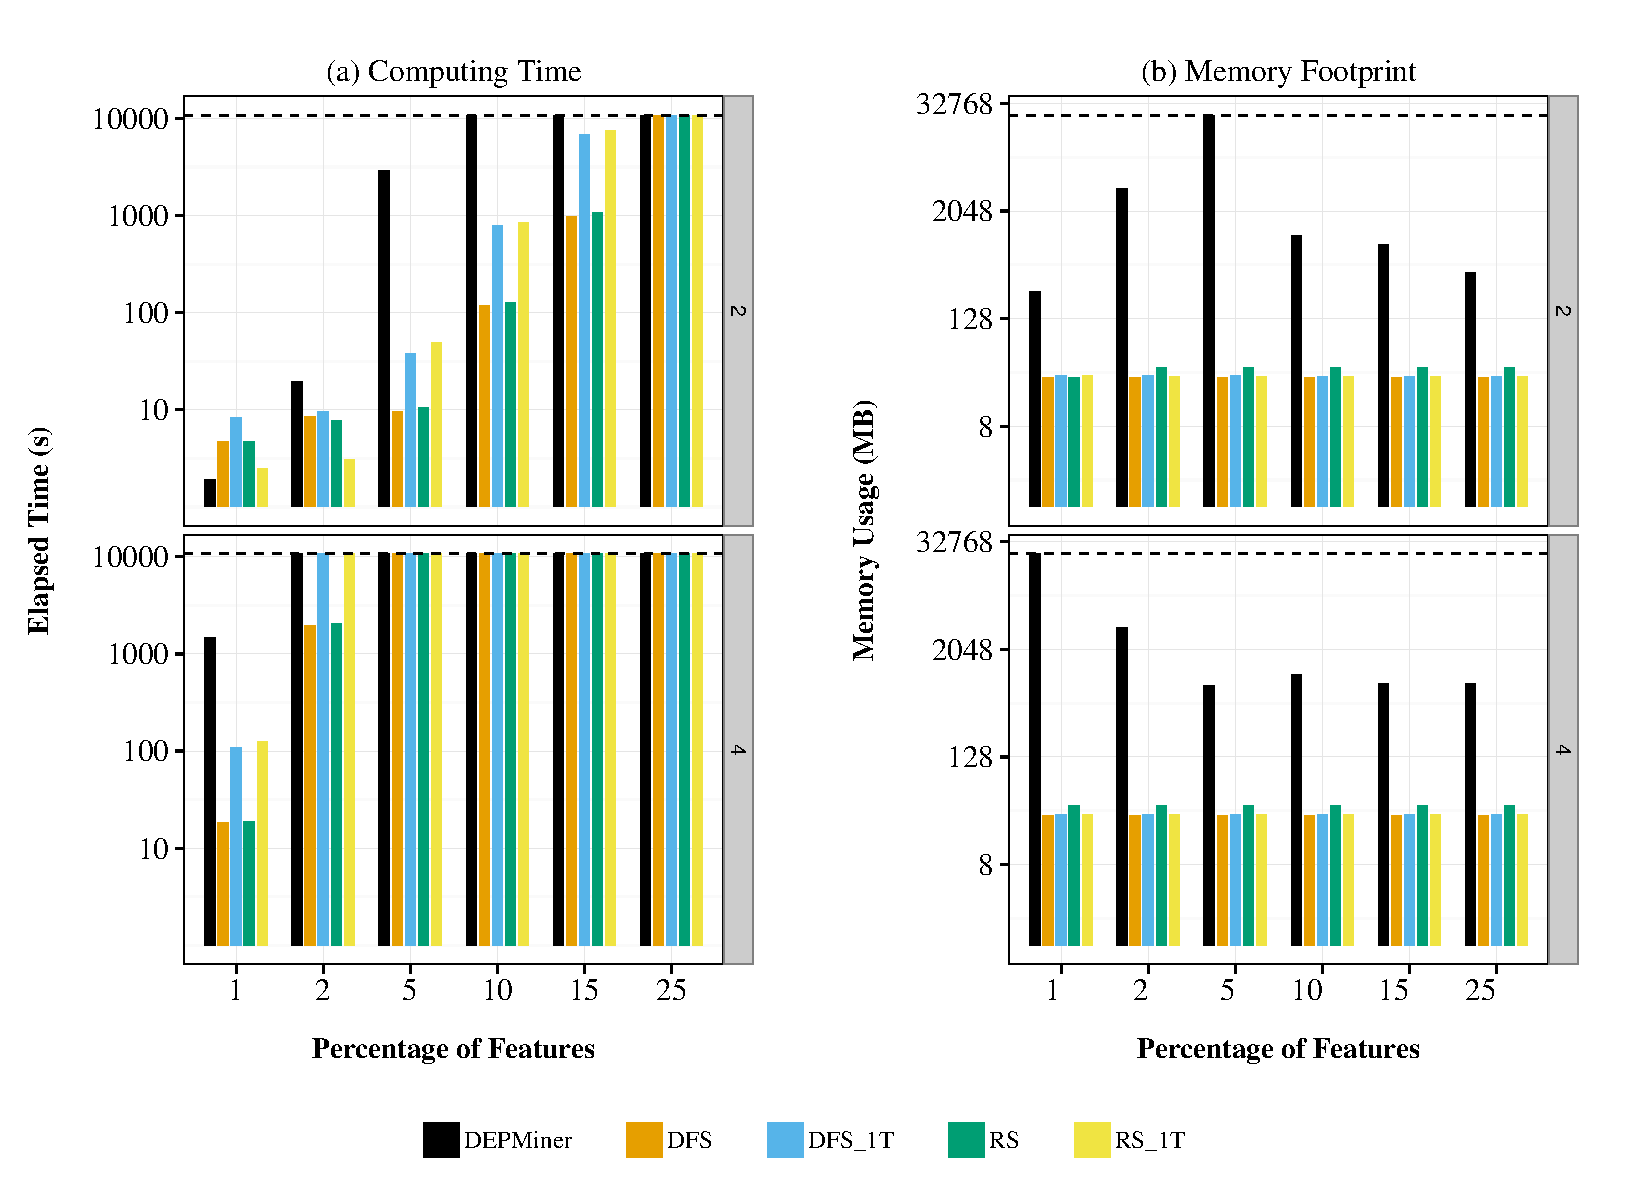
\includegraphics[scale=0.65]{all_aml_ef}
\end{center}
\caption{Performance of the algorithms with the data set ALL-AML discretized with equal frequency.
The suffix `1T' attached to RS and DFS indicates that only one hypergraph was processed a time (the
sequential version); no suffix indicates 8 hypergraphs were processed a time (parallel version).
Numbers on the right-hand side y-axis indicate the number of bins used to discretize the data.}
\label{qcep:fig:allamlef}
\end{figure}

\begin{figure}
\begin{center}
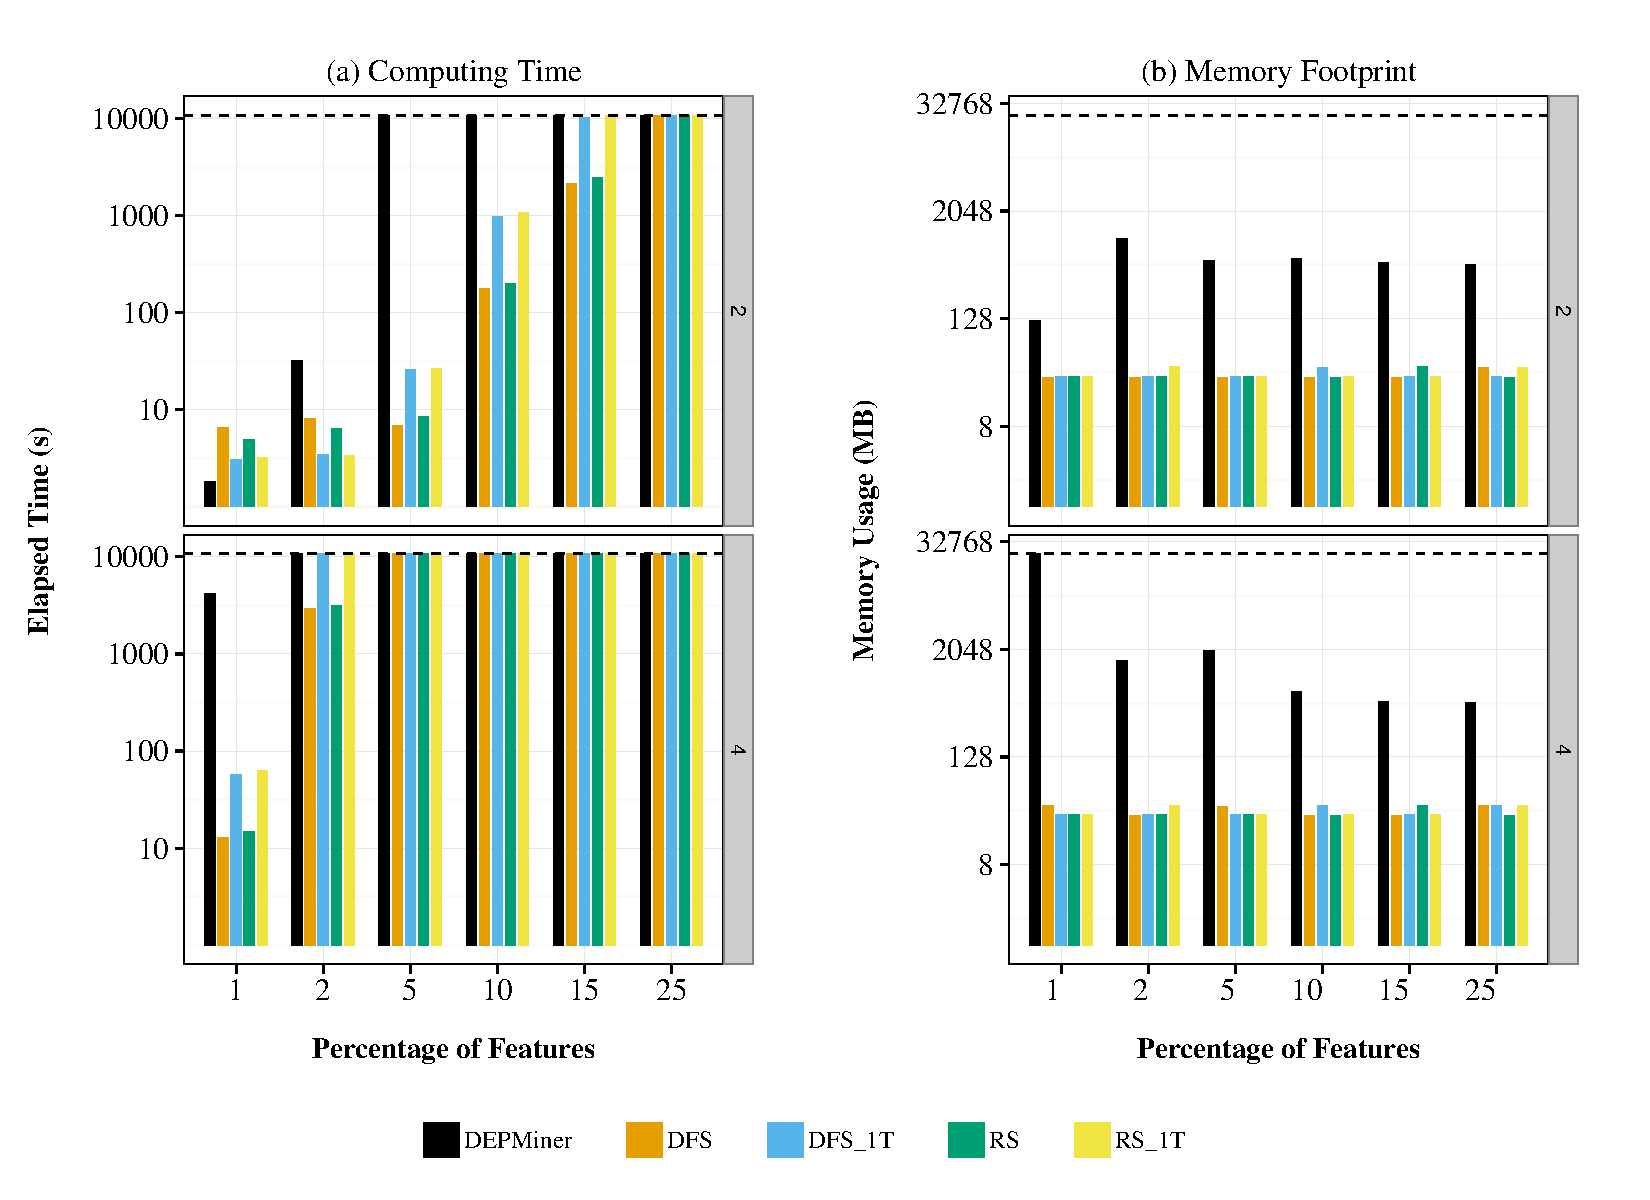
\includegraphics[scale=0.65]{colon_ef}
\end{center}
\caption{Performance of the algorithms with the data set Colon discretized with equal frequency.
The suffix `1T' attached to RS and DFS indicates that only one hypergraph was processed a time (the
sequential version); no suffix indicates 8 hypergraphs were processed a time (parallel version).
Numbers on the right-hand side y-axis indicate the number of bins used to discretize the data.}
\label{qcep:fig:colonef}
\end{figure}

\begin{figure}
\begin{center}
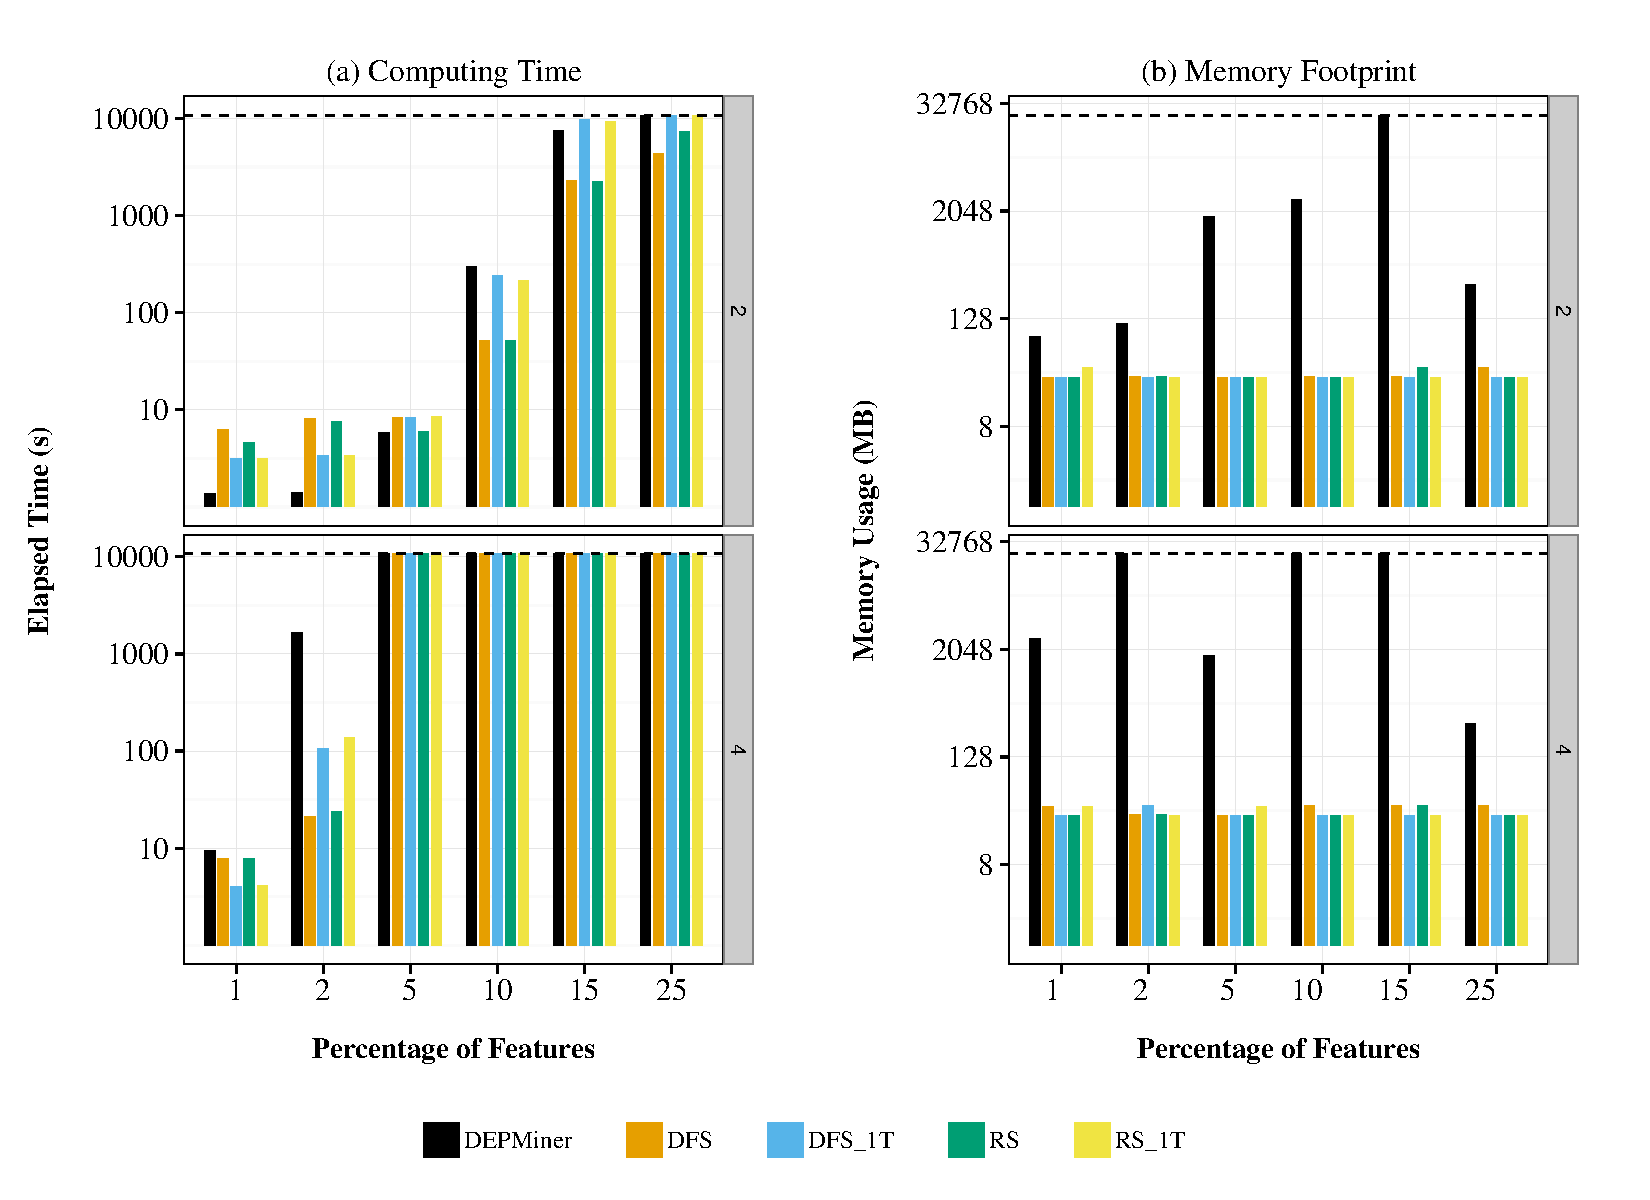
\includegraphics[scale=0.65]{colon_ew}
\end{center}
\caption{Performance of the algorithms with the data set Colon discretized with equal frequency.
The suffix `1T' attached to RS and DFS indicates that only one hypergraph was processed a time (the
sequential version); no suffix indicates 8 hypergraphs were processed a time (parallel version).
Numbers on the right-hand side y-axis indicate the number of bins used to discretize the data.}
\label{qcep:fig:colonef}
\end{figure}

\clearpage
\subsection*{Average datasets}

\begin{figure}[htb]
\begin{center}
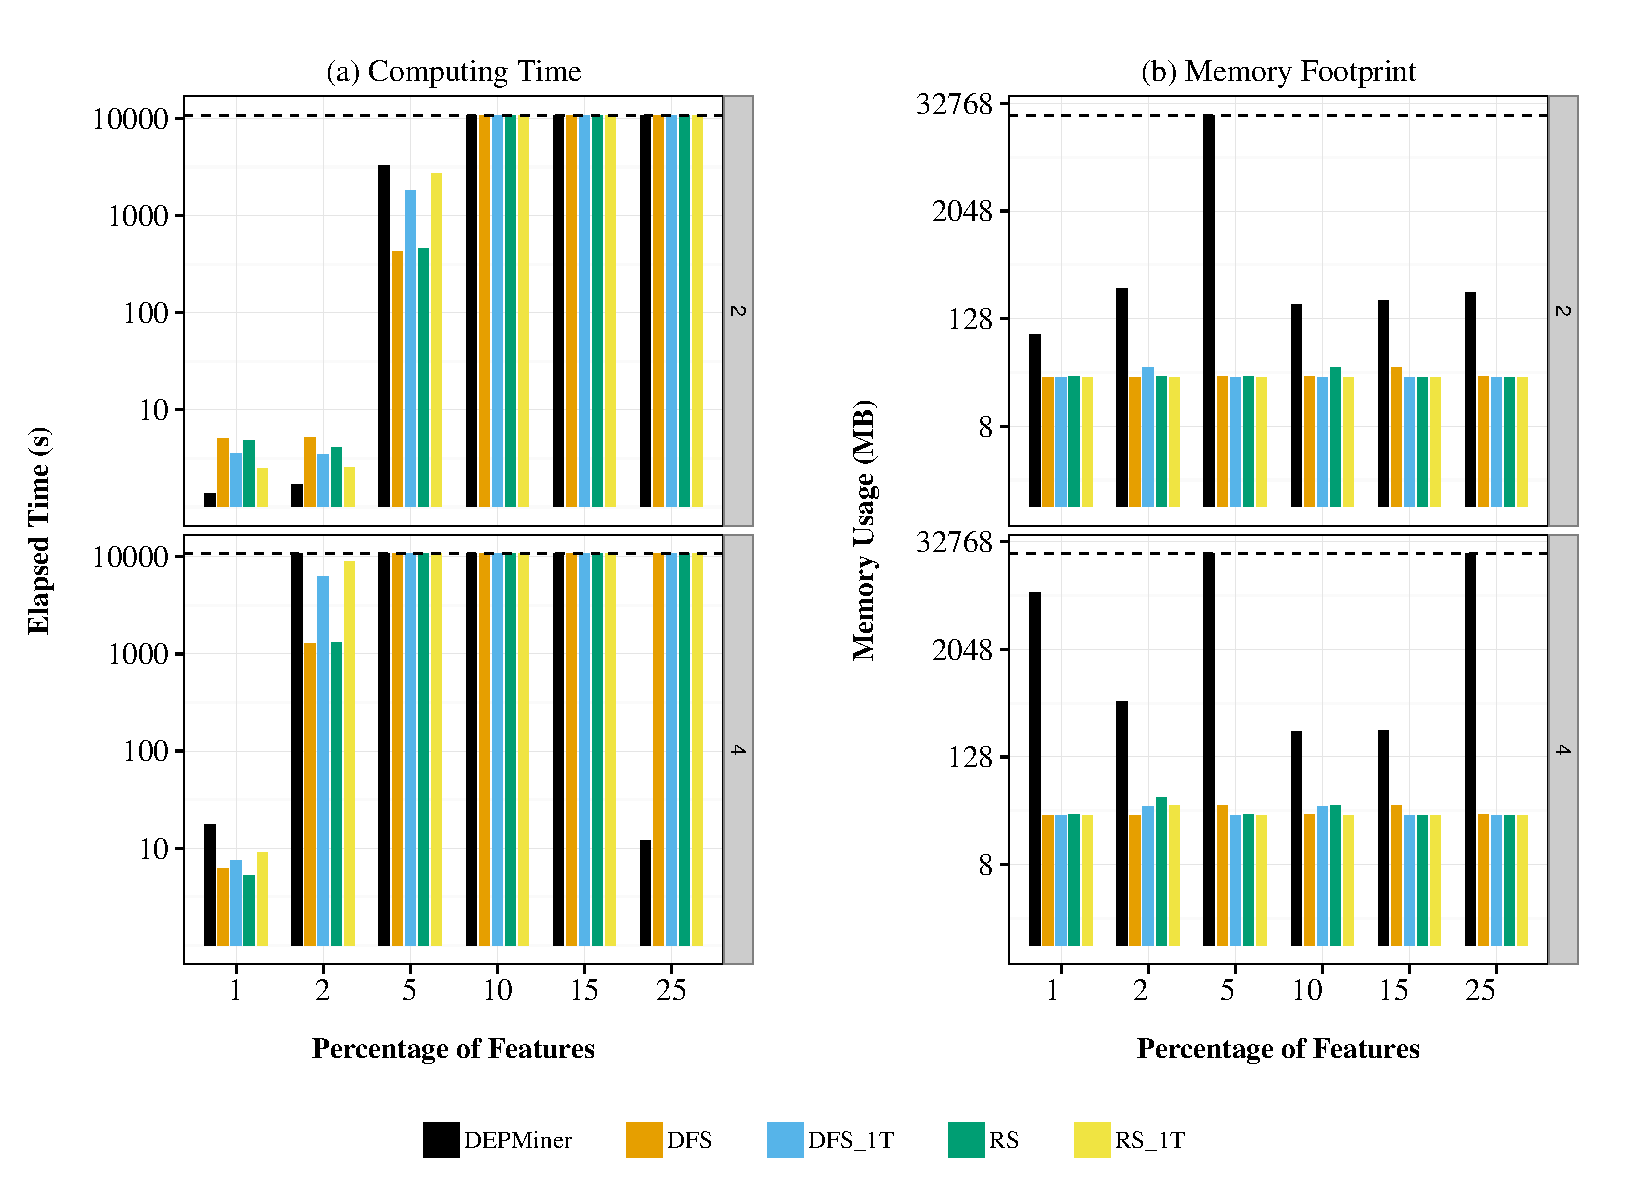
\includegraphics[scale=0.65]{all_aml_ew}
\end{center}
\caption{Performance of the algorithms with the data set ALL-AML discretized with equal frequency.
The suffix `1T' attached to RS and DFS indicates that only one hypergraph was processed a time (the
sequential version); no suffix indicates 8 hypergraphs were processed a time (parallel version).
Numbers on the right-hand side y-axis indicate the number of bins used to discretize the data.}
\label{qcep:fig:allamlef}
\end{figure}


\begin{figure}[htb]
\begin{center}
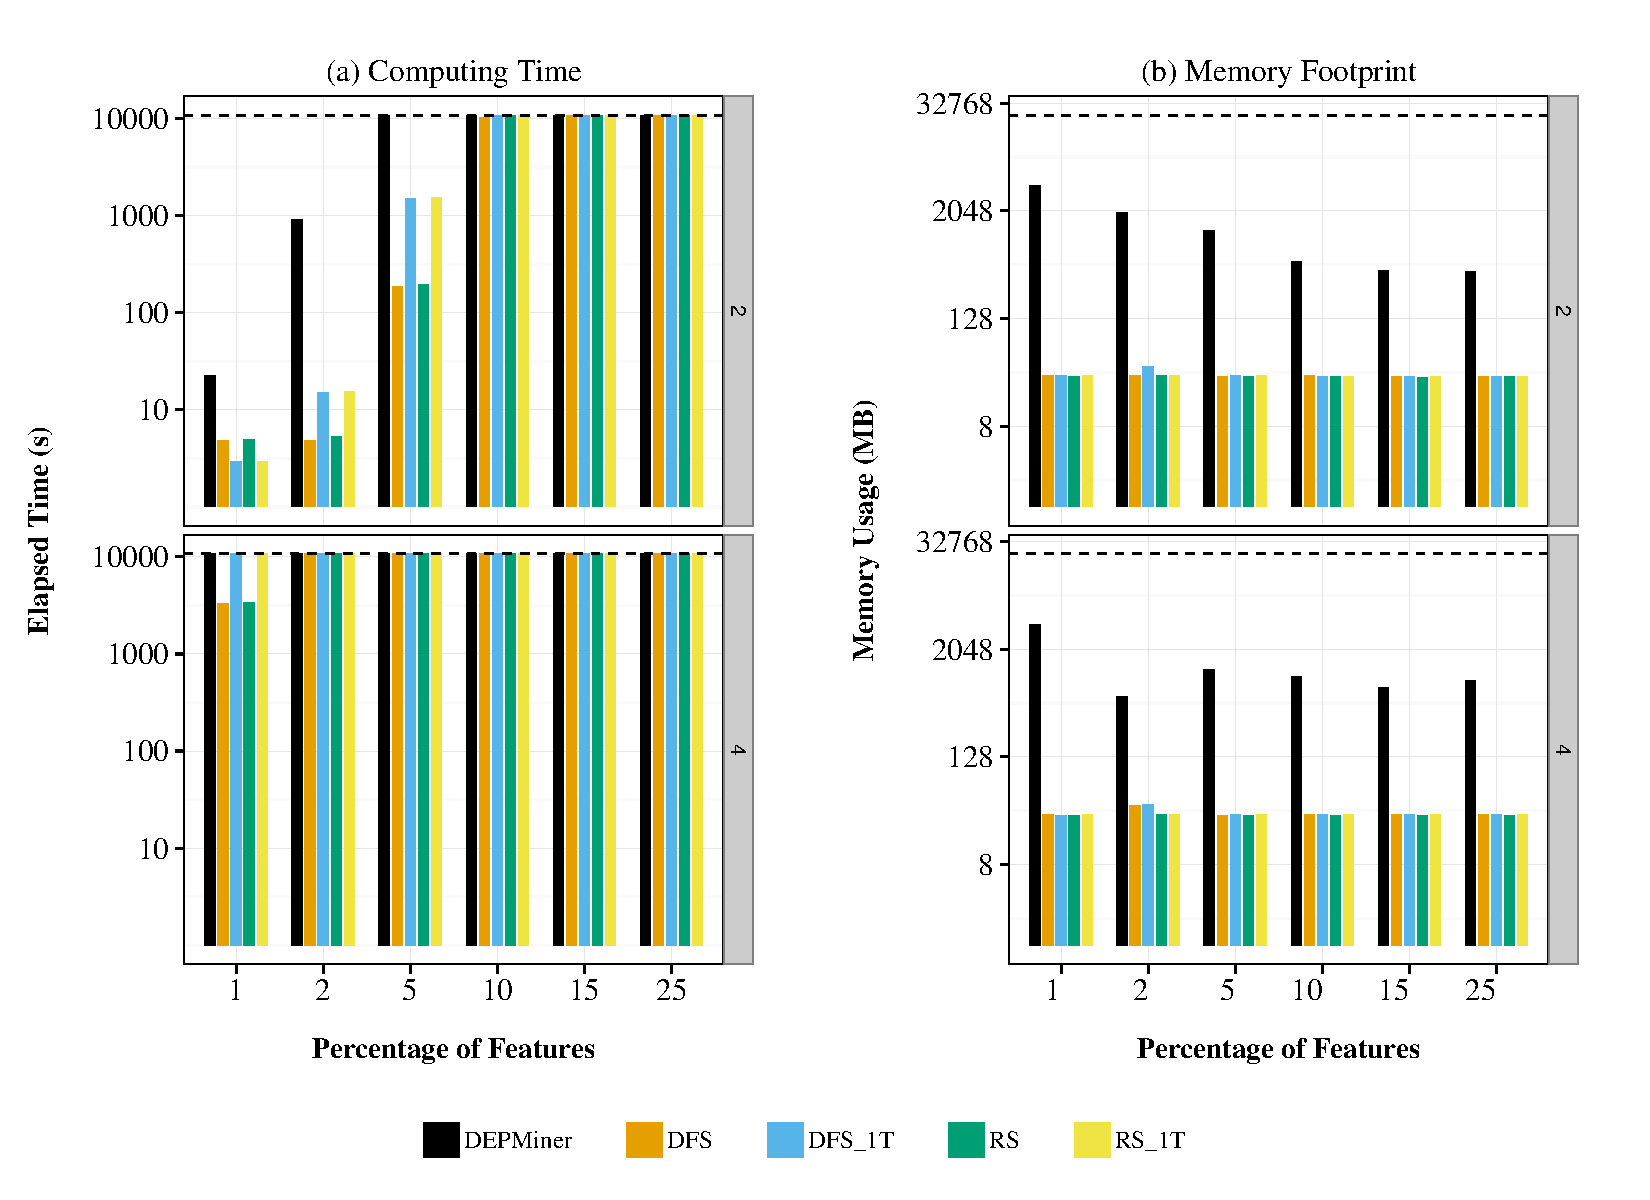
\includegraphics[scale=0.65]{leukemia_ef}
\end{center}
\caption{Performance of the algorithms with the data set Leukemia discretized with equal frequency.
The suffix `1T' attached to RS and DFS indicates that only one hypergraph was processed a time (the
sequential version); no suffix indicates 8 hypergraphs were processed a time (parallel version).
Numbers on the right-hand side y-axis indicate the number of bins used to discretize the data.}
\label{qcep:fig:leukemiaef}
\end{figure}

\begin{figure}
\begin{center}
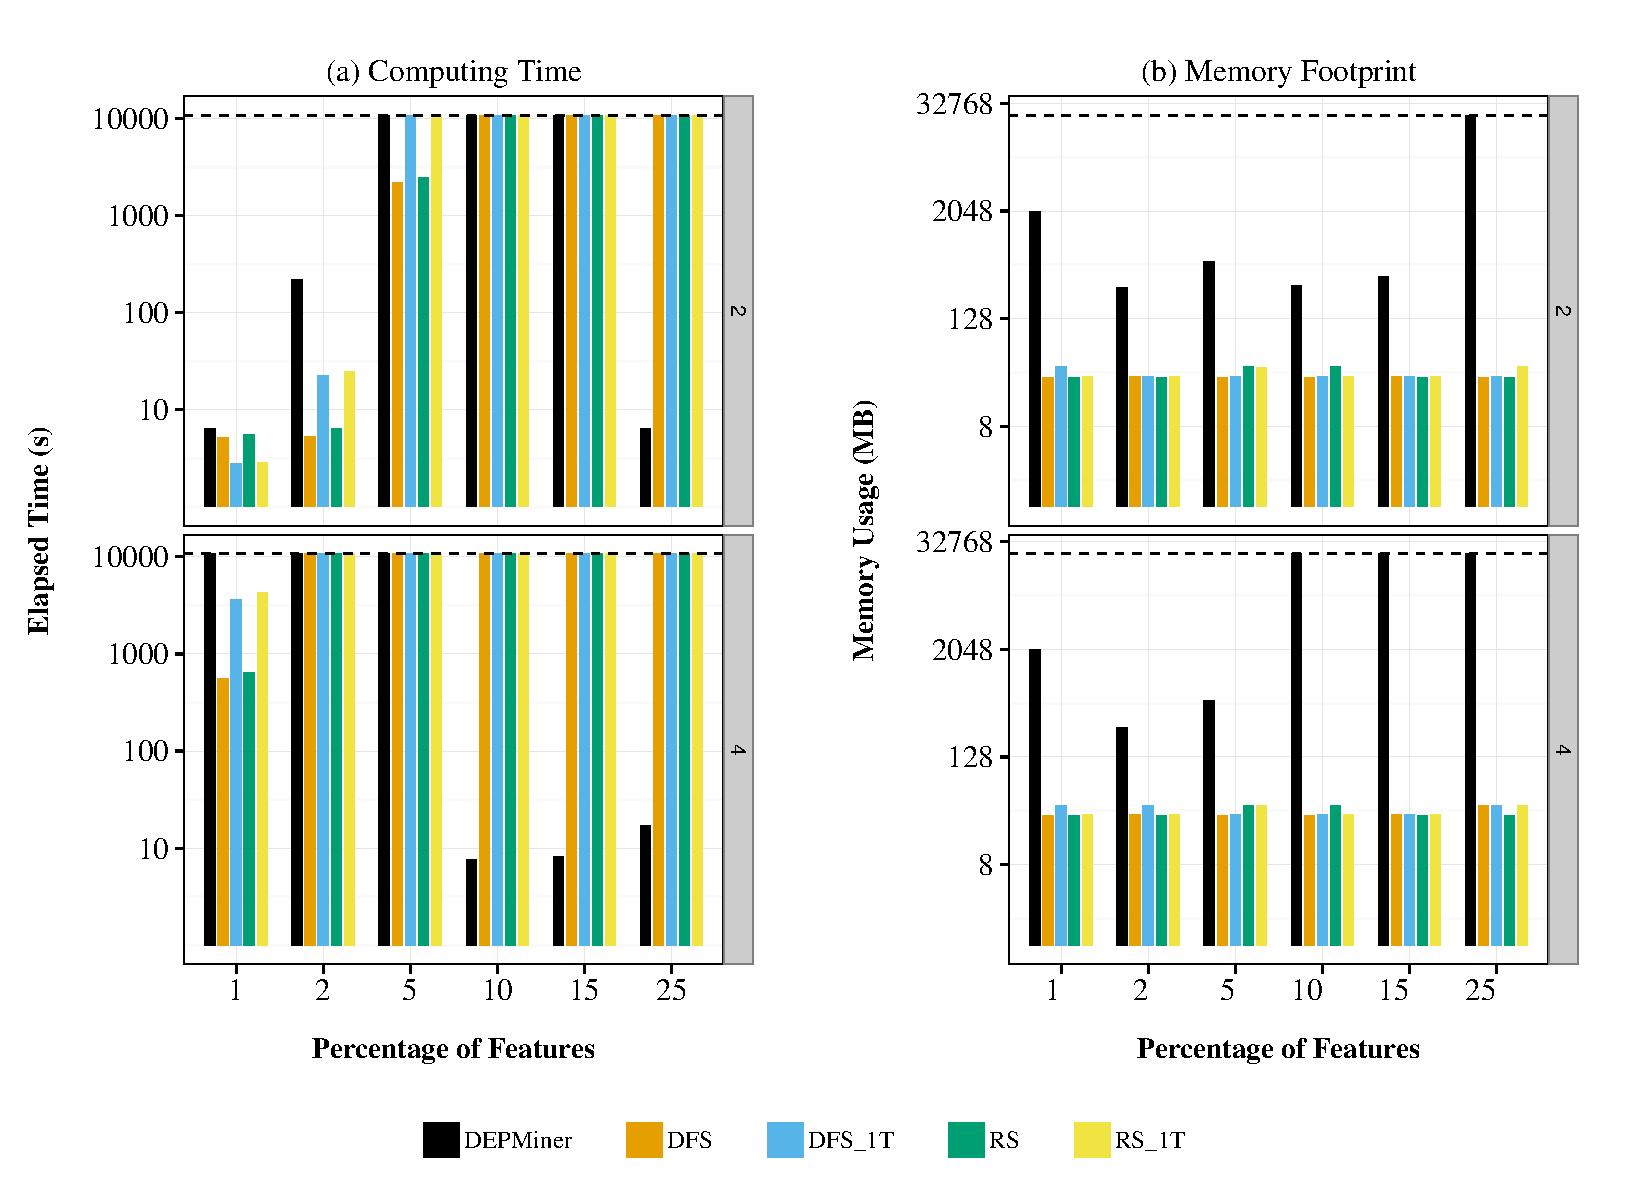
\includegraphics[scale=0.65]{leukemia_ew}
\end{center}
\caption{Performance of the algorithms with the data set Leukemia discretized with equal width.
The suffix `1T' attached to RS and DFS indicates that only one hypergraph was processed a time (the
sequential version); no suffix indicates 8 hypergraphs were processed a time (parallel version).
Numbers on the right-hand side y-axis indicate the number of bins used to discretize the data.}
\label{qcep:fig:leukemiaew}
\end{figure}

\clearpage
\subsection*{Bad datasets}

\begin{figure}[htb]
\begin{center}
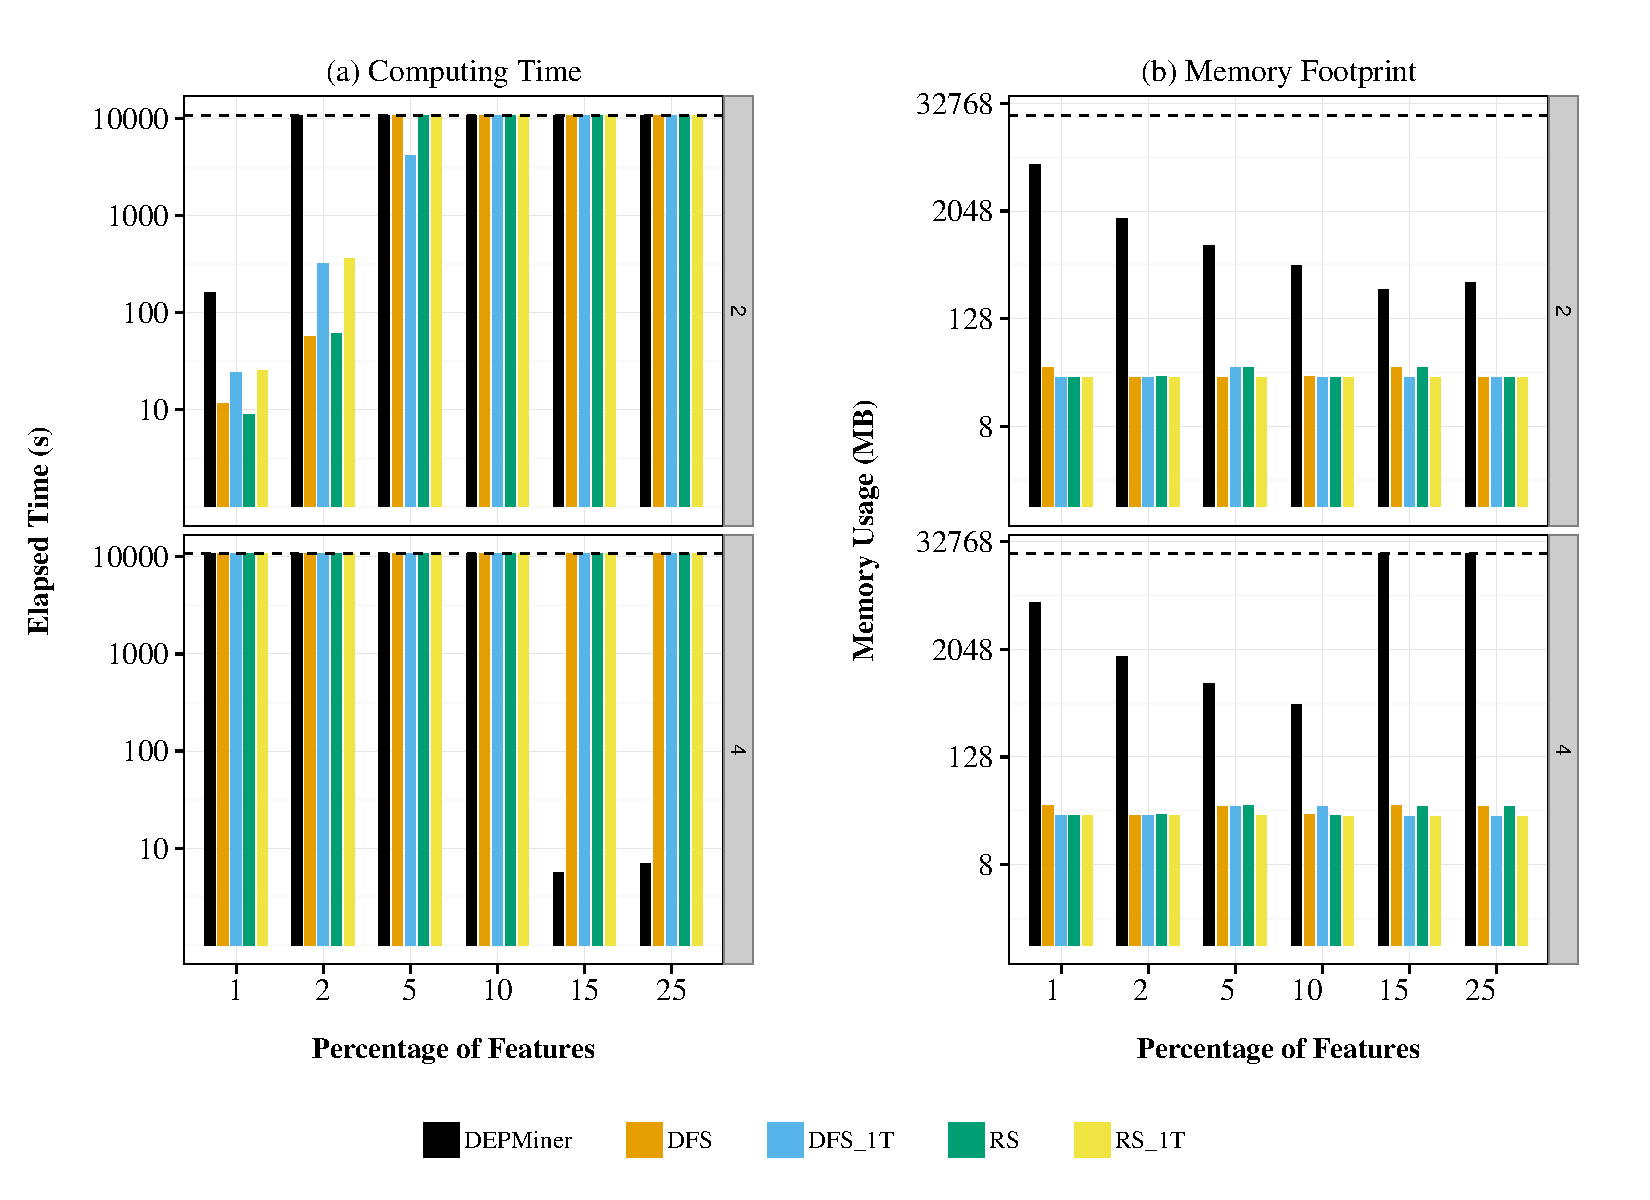
\includegraphics[scale=0.65]{lymphoma_ef}
\end{center}
\caption{Performance of the algorithms with the data set Lymphoma discretized with equal frequency.
The suffix `1T' attached to RS and DFS indicates that only one hypergraph was processed a time (the
sequential version); no suffix indicates 8 hypergraphs were processed a time (parallel version).
Numbers on the right-hand side y-axis indicate the number of bins used to discretize the data.}
\label{qcep:fig:lymphomaef}
\end{figure}

\begin{figure}
\label{qcep:fig:lymphomaew}
\begin{center}
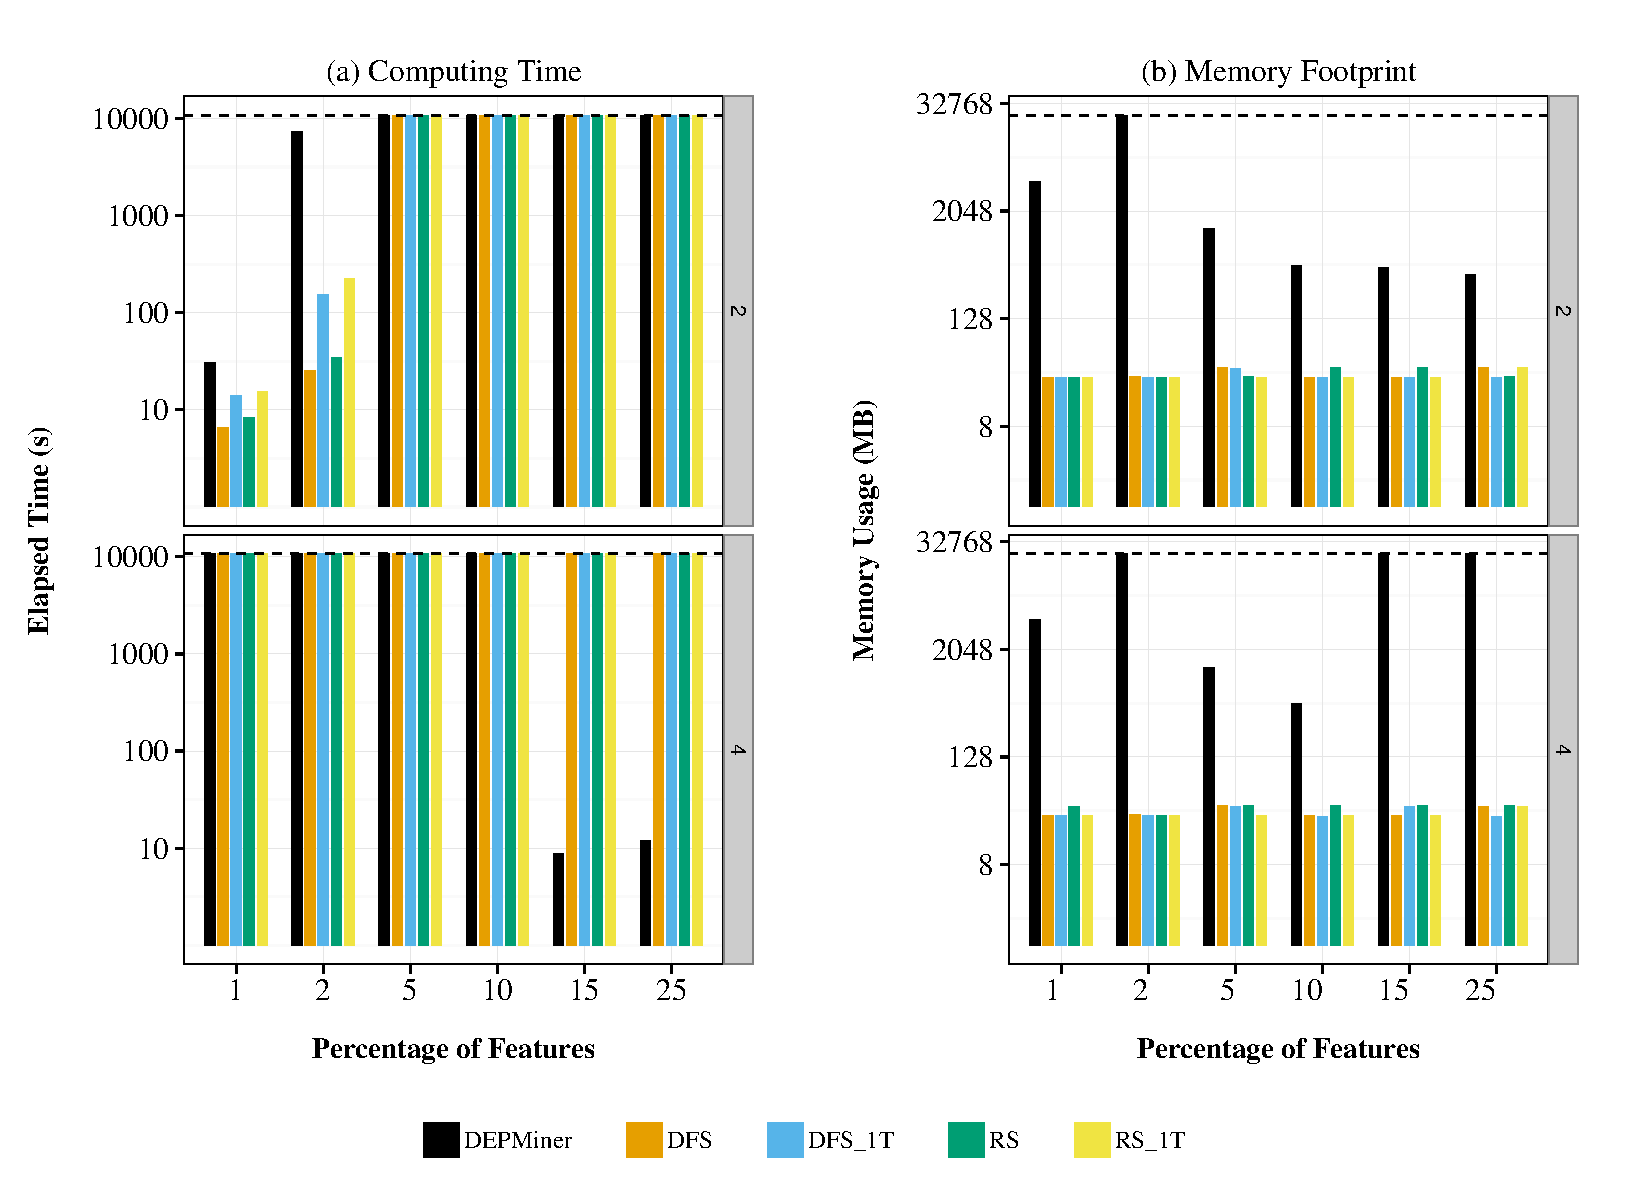
\includegraphics[scale=0.65]{lymphoma_ew}
\end{center}
\caption{Performance of the algorithms with the data set Lymphoma discretized with equal width.
The suffix `1T' attached to RS and DFS indicates that only one hypergraph was processed a time (the
sequential version); no suffix indicates 8 hypergraphs were processed a time (parallel version).
Numbers on the right-hand side y-axis indicate the number of bins used to discretize the data.}
\end{figure}

\clearpage
\section*{Tables with the performance results for mining disjunctive emerging patterns using hypergraphs}
\label{qcep:appendix:tables}

\subsection*{Good datasets}

% latex table generated in R 2.15.1 by xtable 1.7-0 package
% Mon Aug  6 15:43:47 2012
%\begin{longtable}[ht]
\renewcommand{\arraystretch}{1.2}
\begin{center}
\scriptsize
%\begin{tabular}{lrrrrrr}
\begin{longtable}{lrrrrrr}
\caption
{Performance of the algorithms with dataset ALL--AML discretized with equal frequency.
In this table, \emph{Bins} refers to the number of bins used to discretize the data, \emph{Percentage} refers to the percentage of randomly chosen
features, \emph{Status} is the exit status of the program (0 means executed to the end, -15 is timeout, and any other values mean failure to complete),
\emph{Elapsed time} is the time in seconds until the program finished, \emph{System time} is the time in seconds used by the system while the program was running,
\emph{Max. Memory} is the maximum amount of memory used by the program.
}
\\
  \hline
Algorithm & Bins & Percentage & Status & \parbox{1.5cm}{\begin{flushright}Elapsed Time\end{flushright}} 
& \parbox{1.5cm}{\begin{flushright}System Time\end{flushright}} & \parbox{2cm}{\begin{flushright}Max.\\ Memory (MB)\end{flushright}} \\\hline\endfirsthead

\hline
\textit{Table~\thetable\/ (Continued)} & & & & & &  \\[-5mm]
Algorithm & Bins & Percentage & Status & \parbox{1.5cm}{\begin{flushright}Elapsed Time\end{flushright}} 
& \parbox{1.5cm}{\begin{flushright}System Time\end{flushright}} & \parbox{2cm}{\begin{flushright}Max.\\ Memory (MB)\end{flushright}} \\\hline         
\endhead

& & & & & & \\
\multicolumn{7}{r}{\textit{Continued on next page}} \\\hline
\endfoot   

\hline\endlastfoot
\\
DEPMiner     & 2 & 1 &   0 & 0.92 & 0.05 & 258.77 \\ 
  DEPMiner     & 2 & 2 &   0 & 18.44 & 0.71 & 3636.73 \\ 
  DEPMiner     & 2 & 5 &  -6 & 2885.72 & 40.74 & 24153.87 \\ 
  DEPMiner     & 2 & 10 & -15 & 10800.11 & 3.60 & 1083.05 \\ 
  DEPMiner     & 2 & 15 & -15 & 10800.12 & 5.26 & 857.86 \\ 
  DEPMiner     & 2 & 25 & -15 & 10800.10 & 5.36 & 416.31 \\ 
  DEPMiner     & 4 & 1 &  -6 & 1465.61 & 40.16 & 24153.87 \\ 
  DEPMiner     & 4 & 2 & -15 & 10800.11 & 5.37 & 3636.73 \\ 
  DEPMiner     & 4 & 5 & -15 & 10800.00 & 0.23 & 808.58 \\ 
  DEPMiner     & 4 & 10 & -15 & 10800.01 & 4.12 & 1083.05 \\ 
  DEPMiner     & 4 & 15 & -15 & 10800.02 & 5.85 & 857.86 \\ 
  DEPMiner     & 4 & 25 & -15 & 10800.01 & 6.00 & 853.27 \\ 
  DFS     & 2 & 1 &   0 & 3.72 & 0.14 & 28.38 \\ 
  DFS     & 2 & 2 &   0 & 7.57 & 0.61 & 28.39 \\ 
  DFS     & 2 & 5 &   0 & 8.73 & 24.49 & 28.42 \\ 
  DFS     & 2 & 10 &   0 & 116.76 & 25.81 & 28.42 \\ 
  DFS     & 2 & 15 &   0 & 971.83 & 35.60 & 28.42 \\ 
  DFS     & 2 & 25 & -15 & 10800.01 & 35.70 & 28.42 \\ 
  DFS     & 4 & 1 &   0 & 17.23 & 0.41 & 28.38 \\ 
  DFS     & 4 & 2 &   0 & 1963.86 & 24.27 & 28.42 \\ 
  DFS     & 4 & 5 & -15 & 10800.00 & 24.52 & 28.42 \\ 
  DFS     & 4 & 10 & -15 & 10800.00 & 25.84 & 28.42 \\ 
  DFS     & 4 & 15 & -15 & 10800.00 & 35.63 & 28.42 \\ 
  DFS     & 4 & 25 & -15 & 10800.00 & 35.73 & 28.42 \\ 
  DFS\_1T     & 2 & 1 &   0 & 7.37 & 0.10 & 29.20 \\ 
  DFS\_1T     & 2 & 2 &   0 & 8.58 & 0.11 & 29.19 \\ 
  DFS\_1T     & 2 & 5 &   0 & 37.46 & 0.15 & 29.19 \\ 
  DFS\_1T     & 2 & 10 &   0 & 785.58 & 1.17 & 29.16 \\ 
  DFS\_1T     & 2 & 15 &   0 & 6765.42 & 9.87 & 29.17 \\ 
  DFS\_1T     & 2 & 25 & -15 & 10800.00 & 0.03 & 28.97 \\ 
  DFS\_1T     & 4 & 1 &   0 & 107.85 & 0.35 & 29.20 \\ 
  DFS\_1T     & 4 & 2 & -15 & 10800.00 & 0.12 & 29.19 \\ 
  DFS\_1T     & 4 & 5 & -15 & 10800.00 & 0.17 & 29.19 \\ 
  DFS\_1T     & 4 & 10 & -15 & 10800.00 & 1.20 & 29.16 \\ 
  DFS\_1T     & 4 & 15 & -15 & 10800.00 & 9.90 & 29.17 \\ 
  DFS\_1T     & 4 & 25 & -15 & 10800.00 & 0.07 & 28.98 \\ 
%  MTMiner     & 2 & 1 &   0 & 1.42 & 0.12 & 28.56 \\ 
%  MTMiner     & 2 & 2 &   0 & 7.65 & 40.63 & 2856.22 \\ 
%  MTMiner     & 2 & 5 &   0 & 125.45 & 50.34 & 2856.22 \\ 
%  MTMiner     & 2 & 10 &   0 & 3844.42 & 277.96 & 13797.36 \\ 
%  MTMiner     & 2 & 15 & -15 & 10800.04 & 278.08 & 13797.36 \\ 
%  MTMiner     & 2 & 25 & -15 & 10800.07 & 278.20 & 13797.36 \\ 
%  MTMiner     & 4 & 1 &   0 & 715.13 & 40.27 & 2856.22 \\ 
%  MTMiner     & 4 & 2 & -15 & 10800.00 & 40.66 & 2856.22 \\ 
%  MTMiner     & 4 & 5 & -15 & 10800.52 & 50.37 & 2856.22 \\ 
%  MTMiner     & 4 & 10 & -15 & 10800.32 & 277.99 & 13797.36 \\ 
%  MTMiner     & 4 & 15 & -15 & 10800.15 & 278.12 & 13797.36 \\ 
%  MTMiner     & 4 & 25 & -15 & 10800.18 & 278.26 & 13797.36 \\ 
  RS     & 2 & 1 &   0 & 3.77 & 0.16 & 28.39 \\ 
  RS     & 2 & 2 &   0 & 6.82 & 0.63 & 36.20 \\ 
  RS     & 2 & 5 &   0 & 9.53 & 25.65 & 36.20 \\ 
  RS     & 2 & 10 &   0 & 125.77 & 26.99 & 36.20 \\ 
  RS     & 2 & 15 &   0 & 1076.91 & 37.08 & 36.20 \\ 
  RS     & 2 & 25 & -15 & 10800.00 & 37.19 & 36.20 \\ 
  RS     & 4 & 1 &   0 & 17.64 & 0.44 & 36.20 \\ 
  RS     & 4 & 2 &   0 & 2077.86 & 25.43 & 36.20 \\ 
  RS     & 4 & 5 & -15 & 10800.00 & 25.67 & 36.20 \\ 
  RS     & 4 & 10 & -15 & 10800.00 & 27.03 & 36.20 \\ 
  RS     & 4 & 15 & -15 & 10800.00 & 37.11 & 36.20 \\ 
  RS     & 4 & 25 & -15 & 10800.00 & 37.23 & 36.20 \\ 
  RS\_1T     & 2 & 1 &   0 & 1.52 & 0.10 & 29.19 \\ 
  RS\_1T     & 2 & 2 &   0 & 2.07 & 0.08 & 29.16 \\ 
  RS\_1T     & 2 & 5 &   0 & 48.73 & 0.13 & 29.17 \\ 
  RS\_1T     & 2 & 10 &   0 & 852.22 & 1.35 & 29.14 \\ 
  RS\_1T     & 2 & 15 &   0 & 7457.32 & 10.20 & 29.16 \\ 
  RS\_1T     & 2 & 25 & -15 & 10800.00 & 0.02 & 28.95 \\ 
  RS\_1T     & 4 & 1 &   0 & 124.27 & 0.33 & 29.20 \\ 
  RS\_1T     & 4 & 2 & -15 & 10800.00 & 0.12 & 29.16 \\ 
  RS\_1T     & 4 & 5 & -15 & 10800.00 & 0.16 & 29.17 \\ 
  RS\_1T     & 4 & 10 & -15 & 10800.00 & 1.37 & 29.14 \\ 
  RS\_1T     & 4 & 15 & -15 & 10800.00 & 10.22 & 29.16 \\ 
  RS\_1T     & 4 & 25 & -15 & 10800.00 & 0.05 & 28.97 \\ 
%   \hline%\endlastfoot
%\end{tabular}
\end{longtable}
\end{center}
%\end{table}

% latex table generated in R 2.15.1 by xtable 1.7-0 package
% Tue Aug  7 13:31:15 2012
\renewcommand{\arraystretch}{1.2}
\begin{center}
\scriptsize
%\begin{tabular}{lrrrrrr}
\begin{longtable}{lrrrrrr}
\caption
{Performance of the algorithms with dataset Colon discretized with equal width.
In this table, \emph{Bins} refers to the number of bins used to discretize the data, \emph{Percentage} refers to the percentage of randomly chosen
features, \emph{Status} is the exit status of the program (0 means executed to the end, -15 is timeout, and any other values mean failure to complete),
\emph{Elapsed time} is the time in seconds until the program finished, \emph{System time} is the time in seconds used by the system while the program was running,
\emph{Max. Memory} is the maximum amount of memory used by the program.
}
\\
  \hline
Algorithm & Bins & Percentage & Status & \parbox{1.5cm}{\begin{flushright}Elapsed Time\end{flushright}} 
& \parbox{1.5cm}{\begin{flushright}System Time\end{flushright}} & \parbox{2cm}{\begin{flushright}Max.\\ Memory (MB)\end{flushright}} \\\hline\endfirsthead

\hline
\textit{Table~\thetable\/ (Continued)} & & & & & &  \\[-5mm]
Algorithm & Bins & Percentage & Status & \parbox{1.5cm}{\begin{flushright}Elapsed Time\end{flushright}} 
& \parbox{1.5cm}{\begin{flushright}System Time\end{flushright}} & \parbox{2cm}{\begin{flushright}Max.\\ Memory (MB)\end{flushright}} \\\hline         
\endhead

& & & & & & \\
\multicolumn{7}{r}{\textit{Continued on next page}} \\\hline
\endfoot   

\hline\endlastfoot
\\
DEPMiner     & 2 & 1 &   0 & 0.36 & 0.01 & 80.30 \\ 
  DEPMiner     & 2 & 2 &   0 & 0.42 & 0.02 & 111.88 \\ 
  DEPMiner     & 2 & 5 &   0 & 4.87 & 0.36 & 1763.38 \\ 
  DEPMiner     & 2 & 10 &   0 & 301.46 & 17.64 & 2784.94 \\ 
  DEPMiner     & 2 & 15 &  -6 & 7509.21 & 41.15 & 24153.87 \\ 
  DEPMiner     & 2 & 25 & -15 & 10800.00 & 2.70 & 304.86 \\ 
  DEPMiner     & 4 & 1 &   0 & 8.38 & 0.59 & 2704.28 \\ 
  DEPMiner     & 4 & 2 &  -6 & 1673.71 & 31.09 & 24153.87 \\ 
  DEPMiner     & 4 & 5 & -15 & 10800.00 & 2.00 & 1763.38 \\ 
  DEPMiner     & 4 & 10 & -15 & 10800.00 & 19.50 & 24153.87 \\ 
  DEPMiner     & 4 & 15 & -15 & 10800.00 & 41.34 & 24153.87 \\ 
  DEPMiner     & 4 & 25 & -15 & 10800.02 & 2.83 & 304.86 \\ 
  DFS     & 2 & 1 &   0 & 5.32 & 0.18 & 28.16 \\ 
  DFS     & 2 & 2 &   0 & 7.17 & 0.20 & 29.00 \\ 
  DFS     & 2 & 5 &   0 & 7.42 & 0.21 & 28.22 \\ 
  DFS     & 2 & 10 &   0 & 51.13 & 0.70 & 29.00 \\ 
  DFS     & 2 & 15 &   0 & 2304.49 & 16.21 & 29.00 \\ 
  DFS     & 2 & 25 &   0 & 4344.36 & 45.97 & 36.25 \\ 
  DFS     & 4 & 1 &   0 & 6.87 & 0.37 & 36.02 \\ 
  DFS     & 4 & 2 &   0 & 20.14 & 0.54 & 29.00 \\ 
  DFS     & 4 & 5 & -15 & 10800.00 & 0.24 & 28.22 \\ 
  DFS     & 4 & 10 & -15 & 10800.00 & 0.73 & 36.73 \\ 
  DFS     & 4 & 15 & -15 & 10800.00 & 16.26 & 36.70 \\ 
  DFS     & 4 & 25 & -15 & 10800.00 & 46.02 & 36.25 \\ 
  DFS\_1T     & 2 & 1 &   0 & 2.17 & 0.14 & 28.34 \\ 
  DFS\_1T     & 2 & 2 &   0 & 2.37 & 0.15 & 28.38 \\ 
  DFS\_1T     & 2 & 5 &   0 & 7.37 & 0.14 & 28.38 \\ 
  DFS\_1T     & 2 & 10 &   0 & 241.67 & 0.58 & 28.39 \\ 
  DFS\_1T     & 2 & 15 &   0 & 9760.63 & 15.93 & 28.36 \\ 
  DFS\_1T     & 2 & 25 & -15 & 10800.00 & 0.03 & 28.20 \\ 
  DFS\_1T     & 4 & 1 &   0 & 3.02 & 0.28 & 28.38 \\ 
  DFS\_1T     & 4 & 2 &   0 & 105.14 & 0.48 & 36.19 \\ 
  DFS\_1T     & 4 & 5 & -15 & 10800.00 & 0.16 & 28.38 \\ 
  DFS\_1T     & 4 & 10 & -15 & 10800.00 & 0.62 & 28.39 \\ 
  DFS\_1T     & 4 & 15 & -15 & 10800.01 & 15.96 & 28.36 \\ 
  DFS\_1T     & 4 & 25 & -15 & 10800.00 & 0.06 & 28.20 \\ 
%  MTMiner     & 2 & 1 &   0 & 2.07 & 0.16 & 28.94 \\ 
%  MTMiner     & 2 & 2 &   0 & 8.93 & 0.36 & 240.16 \\ 
%  MTMiner     & 2 & 5 &   0 & 1670.00 & 27.59 & 11712.03 \\ 
%  MTMiner     & 2 & 10 & -15 & 10800.00 & 0.03 & 27.97 \\ 
%  MTMiner     & 2 & 15 & -15 & 10800.00 & 0.03 & 27.98 \\ 
%  MTMiner     & 2 & 25 & -15 & 10800.00 & 0.03 & 36.77 \\ 
%  MTMiner     & 4 & 1 &   0 & 33.16 & 1.41 & 214.09 \\ 
%  MTMiner     & 4 & 2 &   0 & 2417.79 & 62.01 & 9498.66 \\ 
%  MTMiner     & 4 & 5 & -15 & 10800.00 & 27.62 & 11712.03 \\ 
%  MTMiner     & 4 & 10 & -15 & 10800.00 & 0.06 & 27.97 \\ 
%  MTMiner     & 4 & 15 & -15 & 10800.00 & 0.06 & 27.98 \\ 
%  MTMiner     & 4 & 25 & -15 & 10800.00 & 0.06 & 36.77 \\ 
  RS     & 2 & 1 &   0 & 3.62 & 0.18 & 28.19 \\ 
  RS     & 2 & 2 &   0 & 6.52 & 0.20 & 29.02 \\ 
  RS     & 2 & 5 &   0 & 4.97 & 0.16 & 28.42 \\ 
  RS     & 2 & 10 &   0 & 51.33 & 0.62 & 28.20 \\ 
  RS     & 2 & 15 &   0 & 2236.99 & 15.81 & 36.25 \\ 
  RS     & 2 & 25 &   0 & 7306.44 & 57.69 & 28.17 \\ 
  RS     & 4 & 1 &   0 & 6.78 & 0.37 & 28.19 \\ 
  RS     & 4 & 2 &   0 & 22.89 & 0.54 & 29.02 \\ 
  RS     & 4 & 5 & -15 & 10800.00 & 0.19 & 28.42 \\ 
  RS     & 4 & 10 & -15 & 10800.00 & 0.64 & 28.20 \\ 
  RS     & 4 & 15 & -15 & 10800.00 & 15.85 & 36.25 \\ 
  RS     & 4 & 25 & -15 & 10800.00 & 57.74 & 28.17 \\ 
  RS\_1T     & 2 & 1 &   0 & 2.17 & 0.13 & 36.02 \\ 
  RS\_1T     & 2 & 2 &   0 & 2.42 & 0.14 & 28.11 \\ 
  RS\_1T     & 2 & 5 &   0 & 7.53 & 0.14 & 28.14 \\ 
  RS\_1T     & 2 & 10 &   0 & 215.59 & 0.58 & 28.14 \\ 
  RS\_1T     & 2 & 15 &   0 & 9284.04 & 15.86 & 28.12 \\ 
  RS\_1T     & 2 & 25 & -15 & 10800.00 & 0.02 & 27.97 \\ 
  RS\_1T     & 4 & 1 &   0 & 3.12 & 0.29 & 36.02 \\ 
  RS\_1T     & 4 & 2 &   0 & 135.33 & 0.44 & 28.16 \\ 
  RS\_1T     & 4 & 5 & -15 & 10800.00 & 0.16 & 35.84 \\ 
  RS\_1T     & 4 & 10 & -15 & 10800.00 & 0.60 & 28.14 \\ 
  RS\_1T     & 4 & 15 & -15 & 10800.02 & 15.90 & 28.12 \\ 
  RS\_1T     & 4 & 25 & -15 & 10800.01 & 0.06 & 27.97 \\ 
\end{longtable}
\end{center}

% latex table generated in R 2.15.1 by xtable 1.7-0 package
% Tue Aug  7 13:31:03 2012
\renewcommand{\arraystretch}{1.2}
\begin{center}
\scriptsize
%\begin{tabular}{lrrrrrr}
\begin{longtable}{lrrrrrr}
\caption
{Performance of the algorithms with dataset Colon discretized with equal frequency.
In this table, \emph{Bins} refers to the number of bins used to discretize the data, \emph{Percentage} refers to the percentage of randomly chosen
features, \emph{Status} is the exit status of the program (0 means executed to the end, -15 is timeout, and any other values mean failure to complete),
\emph{Elapsed time} is the time in seconds until the program finished, \emph{System time} is the time in seconds used by the system while the program was running,
\emph{Max. Memory} is the maximum amount of memory used by the program.
}
\\
  \hline
Algorithm & Bins & Percentage & Status & \parbox{1.5cm}{\begin{flushright}Elapsed Time\end{flushright}} 
& \parbox{1.5cm}{\begin{flushright}System Time\end{flushright}} & \parbox{2cm}{\begin{flushright}Max.\\ Memory (MB)\end{flushright}} \\\hline\endfirsthead

\hline
\textit{Table~\thetable\/ (Continued)} & & & & & &  \\[-5mm]
Algorithm & Bins & Percentage & Status & \parbox{1.5cm}{\begin{flushright}Elapsed Time\end{flushright}} 
& \parbox{1.5cm}{\begin{flushright}System Time\end{flushright}} & \parbox{2cm}{\begin{flushright}Max.\\ Memory (MB)\end{flushright}} \\\hline         
\endhead

& & & & & & \\
\multicolumn{7}{r}{\textit{Continued on next page}} \\\hline
\endfoot   

\hline\endlastfoot
\\
DEPMiner     & 2 & 1 &   0 & 0.81 & 0.03 & 122.12 \\ 
  DEPMiner     & 2 & 2 &   0 & 30.95 & 0.22 & 1001.84 \\ 
  DEPMiner     & 2 & 5 & -15 & 10800.00 & 0.70 & 578.78 \\ 
  DEPMiner     & 2 & 10 & -15 & 10800.00 & 0.16 & 599.16 \\ 
  DEPMiner     & 2 & 15 & -15 & 10800.00 & 0.77 & 537.17 \\ 
  DEPMiner     & 2 & 25 & -15 & 10800.00 & 0.15 & 514.92 \\ 
  DEPMiner     & 4 & 1 &  -6 & 4209.51 & 40.77 & 24153.87 \\ 
  DEPMiner     & 4 & 2 & -15 & 10800.00 & 0.60 & 1528.92 \\ 
  DEPMiner     & 4 & 5 & -15 & 10800.00 & 1.18 & 2014.61 \\ 
  DEPMiner     & 4 & 10 & -15 & 10800.00 & 0.36 & 692.80 \\ 
  DEPMiner     & 4 & 15 & -15 & 10800.00 & 0.88 & 537.17 \\ 
  DEPMiner     & 4 & 25 & -15 & 10800.00 & 0.26 & 514.92 \\ 
  DFS     & 2 & 1 &   0 & 5.52 & 0.19 & 28.42 \\ 
  DFS     & 2 & 2 &   0 & 7.12 & 0.18 & 28.41 \\ 
  DFS     & 2 & 5 &   0 & 5.82 & 0.21 & 28.19 \\ 
  DFS     & 2 & 10 &   0 & 178.59 & 1.63 & 28.20 \\ 
  DFS     & 2 & 15 &   0 & 2143.92 & 16.85 & 28.19 \\ 
  DFS     & 2 & 25 & -15 & 10800.00 & 0.03 & 36.80 \\ 
  DFS     & 4 & 1 &   0 & 11.88 & 0.45 & 36.23 \\ 
  DFS     & 4 & 2 &   0 & 2919.88 & 26.72 & 28.45 \\ 
  DFS     & 4 & 5 & -15 & 10800.00 & 0.25 & 35.92 \\ 
  DFS     & 4 & 10 & -15 & 10800.00 & 1.67 & 28.20 \\ 
  DFS     & 4 & 15 & -15 & 10800.00 & 16.89 & 28.19 \\ 
  DFS     & 4 & 25 & -15 & 10800.00 & 0.07 & 36.80 \\ 
  DFS\_1T     & 2 & 1 &   0 & 2.07 & 0.11 & 28.95 \\ 
  DFS\_1T     & 2 & 2 &   0 & 2.47 & 0.13 & 28.95 \\ 
  DFS\_1T     & 2 & 5 &   0 & 24.90 & 0.16 & 28.98 \\ 
  DFS\_1T     & 2 & 10 &   0 & 969.23 & 1.61 & 36.80 \\ 
  DFS\_1T     & 2 & 15 &   0 & 10320.89 & 16.84 & 29.00 \\ 
  DFS\_1T     & 2 & 25 & -15 & 10800.00 & 0.03 & 28.77 \\ 
  DFS\_1T     & 4 & 1 &   0 & 55.78 & 0.31 & 28.95 \\ 
  DFS\_1T     & 4 & 2 & -15 & 10800.00 & 0.15 & 28.95 \\ 
  DFS\_1T     & 4 & 5 & -15 & 10800.00 & 0.18 & 28.98 \\ 
  DFS\_1T     & 4 & 10 & -15 & 10800.00 & 1.64 & 36.80 \\ 
  DFS\_1T     & 4 & 15 & -15 & 10800.00 & 16.87 & 29.00 \\ 
  DFS\_1T     & 4 & 25 & -15 & 10800.00 & 0.06 & 36.70 \\ 
%  MTMiner     & 2 & 1 &   0 & 2.42 & 0.17 & 28.12 \\ 
%  MTMiner     & 2 & 2 &   0 & 5.77 & 0.43 & 77.91 \\ 
%  MTMiner     & 2 & 5 &   0 & 140.74 & 7.84 & 891.66 \\ 
%  MTMiner     & 2 & 10 &   0 & 8130.27 & 307.29 & 24153.87 \\ 
%  MTMiner     & 2 & 15 & -15 & 10800.92 & 0.03 & 28.16 \\ 
%  MTMiner     & 2 & 25 & 139 & 2238.83 & 51.74 & 24153.87 \\ 
%  MTMiner     & 4 & 1 &   0 & 734.03 & 27.83 & 2718.16 \\ 
%  MTMiner     & 4 & 2 & 139 & 465.18 & 22.59 & 24153.87 \\ 
%  MTMiner     & 4 & 5 & 139 & 562.39 & 27.53 & 24153.87 \\ 
%  MTMiner     & 4 & 10 & 139 & 1347.75 & 325.86 & 24153.87 \\ 
%  MTMiner     & 4 & 15 & 139 & 3867.02 & 50.25 & 24153.87 \\ 
%  MTMiner     & 4 & 25 & 139 & 1995.52 & 78.81 & 24153.87 \\ 
  RS     & 2 & 1 &   0 & 3.97 & 0.17 & 29.02 \\ 
  RS     & 2 & 2 &   0 & 5.37 & 0.20 & 29.02 \\ 
  RS     & 2 & 5 &   0 & 7.47 & 0.21 & 29.00 \\ 
  RS     & 2 & 10 &   0 & 198.57 & 1.64 & 28.20 \\ 
  RS     & 2 & 15 &   0 & 2480.51 & 17.25 & 36.83 \\ 
  RS     & 2 & 25 & -15 & 10800.00 & 0.03 & 28.28 \\ 
  RS     & 4 & 1 &   0 & 13.93 & 0.39 & 29.02 \\ 
  RS     & 4 & 2 &   0 & 3147.75 & 27.19 & 29.02 \\ 
  RS     & 4 & 5 & -15 & 10800.00 & 0.25 & 29.00 \\ 
  RS     & 4 & 10 & -15 & 10800.00 & 1.67 & 28.20 \\ 
  RS     & 4 & 15 & -15 & 10800.00 & 17.29 & 36.83 \\ 
  RS     & 4 & 25 & -15 & 10800.00 & 0.06 & 28.28 \\ 
  RS\_1T     & 2 & 1 &   0 & 2.22 & 0.14 & 28.95 \\ 
  RS\_1T     & 2 & 2 &   0 & 2.42 & 0.13 & 36.84 \\ 
  RS\_1T     & 2 & 5 &   0 & 25.80 & 0.16 & 28.98 \\ 
  RS\_1T     & 2 & 10 &   0 & 1064.47 & 1.68 & 28.97 \\ 
  RS\_1T     & 2 & 15 & -15 & 10800.00 & 0.03 & 28.81 \\ 
  RS\_1T     & 2 & 25 & -15 & 10800.00 & 0.03 & 36.70 \\ 
  RS\_1T     & 4 & 1 &   0 & 62.74 & 0.36 & 28.98 \\ 
  RS\_1T     & 4 & 2 & -15 & 10800.00 & 0.16 & 36.84 \\ 
  RS\_1T     & 4 & 5 & -15 & 10800.00 & 0.19 & 28.98 \\ 
  RS\_1T     & 4 & 10 & -15 & 10800.00 & 1.71 & 28.97 \\ 
  RS\_1T     & 4 & 15 & -15 & 10800.00 & 0.06 & 28.81 \\ 
  RS\_1T     & 4 & 25 & -15 & 10800.00 & 0.05 & 36.70 \\ 
\end{longtable}
\end{center}

%\clearpage

\subsection*{Average datasets}
% latex table generated in R 2.15.1 by xtable 1.7-0 package
% Tue Aug  7 13:16:09 2012
\renewcommand{\arraystretch}{1.2}
\begin{center}
\scriptsize
%\begin{tabular}{lrrrrrr}
\begin{longtable}{lrrrrrr}
\caption
{Performance of the algorithms with dataset ALL--AML discretized with equal width.
In this table, \emph{Bins} refers to the number of bins used to discretize the data, \emph{Percentage} refers to the percentage of randomly chosen
features, \emph{Status} is the exit status of the program (0 means executed to the end, -15 is timeout, and any other values mean failure to complete),
\emph{Elapsed time} is the time in seconds until the program finished, \emph{System time} is the time in seconds used by the system while the program was running,
\emph{Max. Memory} is the maximum amount of memory used by the program.
}
\\
  \hline
Algorithm & Bins & Percentage & Status & \parbox{1.5cm}{\begin{flushright}Elapsed Time\end{flushright}} 
& \parbox{1.5cm}{\begin{flushright}System Time\end{flushright}} & \parbox{2cm}{\begin{flushright}Max.\\ Memory (MB)\end{flushright}} \\\hline\endfirsthead

\hline
\textit{Table~\thetable\/ (Continued)} & & & & & &  \\[-5mm]
Algorithm & Bins & Percentage & Status & \parbox{1.5cm}{\begin{flushright}Elapsed Time\end{flushright}} 
& \parbox{1.5cm}{\begin{flushright}System Time\end{flushright}} & \parbox{2cm}{\begin{flushright}Max.\\ Memory (MB)\end{flushright}} \\\hline         
\endhead

& & & & & & \\
\multicolumn{7}{r}{\textit{Continued on next page}} \\\hline
\endfoot   

\hline\endlastfoot
\\
DEPMiner     & 2 & 1 &   0 & 0.36 & 0.02 & 84.12 \\ 
  DEPMiner     & 2 & 2 &   0 & 0.72 & 0.06 & 279.75 \\ 
  DEPMiner     & 2 & 5 &  -6 & 3312.71 & 39.41 & 24153.87 \\ 
  DEPMiner     & 2 & 10 & -15 & 10800.00 & 0.04 & 183.02 \\ 
  DEPMiner     & 2 & 15 & -15 & 10800.00 & 0.04 & 205.89 \\ 
  DEPMiner     & 2 & 25 & -15 & 10800.00 & 0.10 & 251.70 \\ 
  DEPMiner     & 4 & 1 &   0 & 16.59 & 1.89 & 8794.33 \\ 
  DEPMiner     & 4 & 2 & -15 & 10800.00 & 1.74 & 534.39 \\ 
  DEPMiner     & 4 & 5 & -15 & 10800.00 & 39.50 & 24153.87 \\ 
  DEPMiner     & 4 & 10 & -15 & 10800.00 & 0.13 & 249.58 \\ 
  DEPMiner     & 4 & 15 & -15 & 10800.00 & 0.10 & 255.08 \\ 
  DEPMiner     & 4 & 25 & -11 & 10.88 & 0.24 & 24153.87 \\ 
  DFS     & 2 & 1 &   0 & 4.07 & 0.14 & 28.19 \\ 
  DFS     & 2 & 2 &   0 & 4.22 & 0.14 & 28.16 \\ 
  DFS     & 2 & 5 &   0 & 428.39 & 5.24 & 28.98 \\ 
  DFS     & 2 & 10 & -15 & 10800.00 & 0.03 & 28.80 \\ 
  DFS     & 2 & 15 & -15 & 10800.00 & 0.04 & 36.77 \\ 
  DFS     & 2 & 25 & -15 & 10800.00 & 0.04 & 28.78 \\ 
  DFS     & 4 & 1 &   0 & 5.12 & 0.29 & 28.19 \\ 
  DFS     & 4 & 2 &   0 & 1275.01 & 17.50 & 28.19 \\ 
  DFS     & 4 & 5 & -15 & 10800.00 & 5.28 & 36.73 \\ 
  DFS     & 4 & 10 & -15 & 10800.00 & 0.07 & 28.80 \\ 
  DFS     & 4 & 15 & -15 & 10800.00 & 0.08 & 36.77 \\ 
  DFS     & 4 & 25 & -15 & 10800.01 & 0.08 & 28.80 \\ 
  DFS\_1T     & 2 & 1 &   0 & 2.57 & 0.08 & 28.19 \\ 
  DFS\_1T     & 2 & 2 &   0 & 2.47 & 0.08 & 36.11 \\ 
  DFS\_1T     & 2 & 5 &   0 & 1831.10 & 1.78 & 28.23 \\ 
  DFS\_1T     & 2 & 10 & -15 & 10800.00 & 0.01 & 28.00 \\ 
  DFS\_1T     & 2 & 15 & -15 & 10800.00 & 0.01 & 28.00 \\ 
  DFS\_1T     & 2 & 25 & -15 & 10800.00 & 0.01 & 27.95 \\ 
  DFS\_1T     & 4 & 1 &   0 & 6.43 & 0.16 & 28.20 \\ 
  DFS\_1T     & 4 & 2 &   0 & 6312.16 & 5.85 & 36.11 \\ 
  DFS\_1T     & 4 & 5 & -15 & 10800.00 & 1.81 & 28.23 \\ 
  DFS\_1T     & 4 & 10 & -15 & 10800.00 & 0.03 & 35.95 \\ 
  DFS\_1T     & 4 & 15 & -15 & 10800.00 & 0.03 & 28.00 \\ 
  DFS\_1T     & 4 & 25 & -15 & 10800.00 & 0.03 & 28.00 \\ 
%  MTMiner     & 2 & 1 &   0 & 1.57 & 0.09 & 28.12 \\ 
%  MTMiner     & 2 & 2 &   0 & 5.48 & 0.28 & 62.97 \\ 
%  MTMiner     & 2 & 5 & 139 & 6498.88 & 208.87 & 24153.87 \\ 
%  MTMiner     & 2 & 10 & 139 & 580.39 & 21.24 & 24153.87 \\ 
%  MTMiner     & 2 & 15 & 139 & 823.84 & 21.17 & 24153.87 \\ 
%  MTMiner     & 2 & 25 & 139 & 1452.83 & 20.54 & 24153.87 \\ 
%  MTMiner     & 4 & 1 &   0 & 154.77 & 5.29 & 984.08 \\ 
%  MTMiner     & 4 & 2 & 139 & 527.25 & 24.21 & 24153.87 \\ 
%  MTMiner     & 4 & 5 & 139 & 718.90 & 228.66 & 24153.87 \\ 
%  MTMiner     & 4 & 10 & 139 & 1517.03 & 40.70 & 24153.87 \\ 
%  MTMiner     & 4 & 15 & 139 & 1856.52 & 40.65 & 24153.87 \\ 
%  MTMiner     & 4 & 25 & 139 & 2146.16 & 39.87 & 24153.87 \\ 
  RS     & 2 & 1 &   0 & 3.82 & 0.16 & 28.98 \\ 
  RS     & 2 & 2 &   0 & 3.07 & 0.14 & 29.00 \\ 
  RS     & 2 & 5 &   0 & 460.63 & 3.17 & 29.00 \\ 
  RS     & 2 & 10 & -15 & 10800.00 & 0.04 & 36.77 \\ 
  RS     & 2 & 15 & -15 & 10800.00 & 0.03 & 27.97 \\ 
  RS     & 2 & 25 & -15 & 10800.00 & 0.03 & 28.19 \\ 
  RS     & 4 & 1 &   0 & 4.22 & 0.31 & 29.00 \\ 
  RS     & 4 & 2 &   0 & 1304.14 & 17.57 & 44.84 \\ 
  RS     & 4 & 5 & -15 & 10800.00 & 3.20 & 29.00 \\ 
  RS     & 4 & 10 & -15 & 10800.00 & 0.07 & 36.77 \\ 
  RS     & 4 & 15 & -15 & 10800.00 & 0.06 & 27.97 \\ 
  RS     & 4 & 25 & -15 & 10800.00 & 0.07 & 28.22 \\ 
  RS\_1T     & 2 & 1 &   0 & 1.47 & 0.09 & 28.39 \\ 
  RS\_1T     & 2 & 2 &   0 & 1.57 & 0.08 & 28.36 \\ 
  RS\_1T     & 2 & 5 &   0 & 2732.66 & 5.31 & 28.38 \\ 
  RS\_1T     & 2 & 10 & -15 & 10800.00 & 0.02 & 28.16 \\ 
  RS\_1T     & 2 & 15 & -15 & 10800.00 & 0.03 & 28.17 \\ 
  RS\_1T     & 2 & 25 & -15 & 10800.00 & 0.03 & 28.14 \\ 
  RS\_1T     & 4 & 1 &   0 & 8.08 & 0.21 & 28.39 \\ 
  RS\_1T     & 4 & 2 &   0 & 8954.84 & 17.68 & 36.19 \\ 
  RS\_1T     & 4 & 5 & -15 & 10800.00 & 5.33 & 28.38 \\ 
  RS\_1T     & 4 & 10 & -15 & 10800.00 & 0.06 & 28.16 \\ 
  RS\_1T     & 4 & 15 & -15 & 10800.00 & 0.05 & 28.17 \\ 
  RS\_1T     & 4 & 25 & -15 & 10800.00 & 0.05 & 28.14 \\ 
\end{longtable}
\end{center}

% latex table generated in R 2.15.1 by xtable 1.7-0 package
% Tue Aug  7 13:45:18 2012
\renewcommand{\arraystretch}{1.2}
\begin{center}
\scriptsize
%\begin{tabular}{lrrrrrr}
\begin{longtable}{lrrrrrr}
\caption
{Performance of the algorithms with dataset Leukemia discretized with equal frequency.
In this table, \emph{Bins} refers to the number of bins used to discretize the data, \emph{Percentage} refers to the percentage of randomly chosen
features, \emph{Status} is the exit status of the program (0 means executed to the end, -15 is timeout, and any other values mean failure to complete),
\emph{Elapsed time} is the time in seconds until the program finished, \emph{System time} is the time in seconds used by the system while the program was running,
\emph{Max. Memory} is the maximum amount of memory used by the program.
}
\\
  \hline
Algorithm & Bins & Percentage & Status & \parbox{1.5cm}{\begin{flushright}Elapsed Time\end{flushright}} 
& \parbox{1.5cm}{\begin{flushright}System Time\end{flushright}} & \parbox{2cm}{\begin{flushright}Max.\\ Memory (MB)\end{flushright}} \\\hline\endfirsthead

\hline
\textit{Table~\thetable\/ (Continued)} & & & & & &  \\[-5mm]
Algorithm & Bins & Percentage & Status & \parbox{1.5cm}{\begin{flushright}Elapsed Time\end{flushright}} 
& \parbox{1.5cm}{\begin{flushright}System Time\end{flushright}} & \parbox{2cm}{\begin{flushright}Max.\\ Memory (MB)\end{flushright}} \\\hline         
\endhead

& & & & & & \\
\multicolumn{7}{r}{\textit{Continued on next page}} \\\hline
\endfoot   

\hline\endlastfoot
\\
DEPMiner     & 2 & 1 &   0 & 21.54 & 0.86 & 3916.41 \\ 
  DEPMiner     & 2 & 2 &   0 & 915.51 & 18.57 & 1939.55 \\ 
  DEPMiner     & 2 & 5 & -15 & 10800.02 & 0.68 & 1224.41 \\ 
  DEPMiner     & 2 & 10 & -15 & 10800.01 & 0.60 & 556.47 \\ 
  DEPMiner     & 2 & 15 & -15 & 10800.02 & 0.51 & 443.23 \\ 
  DEPMiner     & 2 & 25 & -15 & 10800.02 & 0.55 & 424.80 \\ 
  DEPMiner     & 4 & 1 & -15 & 10800.00 & 1.56 & 3916.41 \\ 
  DEPMiner     & 4 & 2 & -15 & 10800.00 & 0.37 & 606.39 \\ 
  DEPMiner     & 4 & 5 & -15 & 10800.02 & 1.43 & 1224.41 \\ 
  DEPMiner     & 4 & 10 & -15 & 10800.01 & 1.48 & 1024.34 \\ 
  DEPMiner     & 4 & 15 & -15 & 10800.01 & 1.25 & 754.22 \\ 
  DEPMiner     & 4 & 25 & -15 & 10800.02 & 1.32 & 907.81 \\ 
  DFS     & 2 & 1 &   0 & 3.87 & 0.14 & 29.23 \\ 
  DFS     & 2 & 2 &   0 & 3.82 & 0.16 & 29.27 \\ 
  DFS     & 2 & 5 &   0 & 185.39 & 0.96 & 28.41 \\ 
  DFS     & 2 & 10 &   0 & 10233.47 & 84.28 & 29.22 \\ 
  DFS     & 2 & 15 & -15 & 10800.00 & 0.03 & 29.08 \\ 
  DFS     & 2 & 25 & -15 & 10800.00 & 0.03 & 29.02 \\ 
  DFS     & 4 & 1 &   0 & 3307.54 & 39.99 & 29.23 \\ 
  DFS     & 4 & 2 & -15 & 10800.00 & 0.19 & 36.97 \\ 
  DFS     & 4 & 5 & -15 & 10800.00 & 1.00 & 28.41 \\ 
  DFS     & 4 & 10 & -15 & 10800.00 & 84.32 & 29.22 \\ 
  DFS     & 4 & 15 & -15 & 10800.01 & 0.07 & 29.08 \\ 
  DFS     & 4 & 25 & -15 & 10800.00 & 0.08 & 29.02 \\ 
  DFS\_1T     & 2 & 1 &   0 & 1.97 & 0.09 & 29.16 \\ 
  DFS\_1T     & 2 & 2 &   0 & 14.13 & 0.10 & 37.05 \\ 
  DFS\_1T     & 2 & 5 &   0 & 1501.27 & 2.05 & 29.19 \\ 
  DFS\_1T     & 2 & 10 & -15 & 10800.00 & 0.02 & 28.98 \\ 
  DFS\_1T     & 2 & 15 & -15 & 10800.01 & 0.02 & 28.97 \\ 
  DFS\_1T     & 2 & 25 & -15 & 10800.01 & 0.03 & 28.97 \\ 
  DFS\_1T     & 4 & 1 & -15 & 10800.00 & 0.02 & 28.47 \\ 
  DFS\_1T     & 4 & 2 & -15 & 10800.00 & 0.12 & 37.05 \\ 
  DFS\_1T     & 4 & 5 & -15 & 10800.01 & 0.75 & 29.20 \\ 
  DFS\_1T     & 4 & 10 & -15 & 10800.01 & 2.39 & 29.23 \\ 
  DFS\_1T     & 4 & 15 & -15 & 10800.01 & 0.04 & 28.98 \\ 
  DFS\_1T     & 4 & 25 & -15 & 10800.01 & 0.06 & 28.97 \\ 
%  MTMiner     & 2 & 1 &   0 & 3.02 & 0.29 & 29.19 \\ 
%  MTMiner     & 2 & 2 &   0 & 43.78 & 3.82 & 179.95 \\ 
%  MTMiner     & 2 & 5 &   0 & 5329.05 & 311.69 & 11662.52 \\ 
%  MTMiner     & 2 & 10 & -15 & 10800.00 & 0.03 & 28.14 \\ 
%  MTMiner     & 2 & 15 & -15 & 10800.00 & 0.04 & 28.17 \\ 
%  MTMiner     & 2 & 25 & -15 & 10800.00 & 0.03 & 28.97 \\ 
%  MTMiner     & 4 & 1 & -15 & 10800.00 & 0.32 & 29.19 \\ 
%  MTMiner     & 4 & 2 & -15 & 10800.00 & 3.85 & 179.95 \\ 
%  MTMiner     & 4 & 5 & -15 & 10800.00 & 311.72 & 11662.52 \\ 
%  MTMiner     & 4 & 10 & -15 & 10800.00 & 0.05 & 28.16 \\ 
%  MTMiner     & 4 & 15 & -15 & 10800.00 & 0.07 & 28.17 \\ 
%  MTMiner     & 4 & 25 & -15 & 10800.00 & 0.07 & 28.98 \\ 
  RS     & 2 & 1 &   0 & 3.92 & 0.14 & 28.39 \\ 
  RS     & 2 & 2 &   0 & 4.37 & 0.18 & 29.22 \\ 
  RS     & 2 & 5 &   0 & 195.30 & 1.63 & 28.44 \\ 
  RS     & 2 & 10 & -15 & 10800.00 & 0.04 & 28.50 \\ 
  RS     & 2 & 15 & -15 & 10800.00 & 0.04 & 28.27 \\ 
  RS     & 2 & 25 & -15 & 10800.00 & 0.03 & 28.39 \\ 
  RS     & 4 & 1 &   0 & 3395.04 & 24.56 & 28.39 \\ 
  RS     & 4 & 2 & -15 & 10800.00 & 0.21 & 29.22 \\ 
  RS     & 4 & 5 & -15 & 10800.00 & 1.67 & 28.44 \\ 
  RS     & 4 & 10 & -15 & 10800.00 & 0.07 & 28.50 \\ 
  RS     & 4 & 15 & -15 & 10800.00 & 0.08 & 28.27 \\ 
  RS     & 4 & 25 & -15 & 10800.00 & 0.03 & 28.38 \\ 
  RS\_1T     & 2 & 1 &   0 & 1.97 & 0.09 & 29.22 \\ 
  RS\_1T     & 2 & 2 &   0 & 14.33 & 0.12 & 29.19 \\ 
  RS\_1T     & 2 & 5 &   0 & 1547.98 & 2.85 & 29.23 \\ 
  RS\_1T     & 2 & 10 & -15 & 10800.00 & 0.03 & 29.00 \\ 
  RS\_1T     & 2 & 15 & -15 & 10800.01 & 0.02 & 28.95 \\ 
  RS\_1T     & 2 & 25 & -15 & 10800.01 & 0.02 & 28.97 \\ 
  RS\_1T     & 4 & 1 & -15 & 10800.00 & 0.03 & 29.03 \\ 
  RS\_1T     & 4 & 2 & -15 & 10800.00 & 0.14 & 29.19 \\ 
  RS\_1T     & 4 & 5 & -15 & 10800.01 & 0.46 & 29.20 \\ 
  RS\_1T     & 4 & 10 & -15 & 10800.01 & 2.50 & 29.22 \\ 
  RS\_1T     & 4 & 15 & -15 & 10800.00 & 0.04 & 28.97 \\ 
  RS\_1T     & 4 & 25 & -15 & 10800.01 & 0.04 & 28.98 \\ 
\end{longtable}
\end{center}

% latex table generated in R 2.15.1 by xtable 1.7-0 package
% Tue Aug  7 13:44:44 2012
\renewcommand{\arraystretch}{1.2}
\begin{center}
\scriptsize
%\begin{tabular}{lrrrrrr}
\begin{longtable}{lrrrrrr}
\caption
{Performance of the algorithms with dataset Leukemia discretized with equal width.
In this table, \emph{Bins} refers to the number of bins used to discretize the data, \emph{Percentage} refers to the percentage of randomly chosen
features, \emph{Status} is the exit status of the program (0 means executed to the end, -15 is timeout, and any other values mean failure to complete),
\emph{Elapsed time} is the time in seconds until the program finished, \emph{System time} is the time in seconds used by the system while the program was running,
\emph{Max. Memory} is the maximum amount of memory used by the program.
}
\\
  \hline
Algorithm & Bins & Percentage & Status & \parbox{1.5cm}{\begin{flushright}Elapsed Time\end{flushright}} 
& \parbox{1.5cm}{\begin{flushright}System Time\end{flushright}} & \parbox{2cm}{\begin{flushright}Max.\\ Memory (MB)\end{flushright}} \\\hline\endfirsthead

\hline
\textit{Table~\thetable\/ (Continued)} & & & & & &  \\[-5mm]
Algorithm & Bins & Percentage & Status & \parbox{1.5cm}{\begin{flushright}Elapsed Time\end{flushright}} 
& \parbox{1.5cm}{\begin{flushright}System Time\end{flushright}} & \parbox{2cm}{\begin{flushright}Max.\\ Memory (MB)\end{flushright}} \\\hline         
\endhead

& & & & & & \\
\multicolumn{7}{r}{\textit{Continued on next page}} \\\hline
\endfoot   

\hline\endlastfoot
\\
DEPMiner     & 2 & 1 &   0 & 5.47 & 0.41 & 2018.00 \\ 
  DEPMiner     & 2 & 2 &   0 & 221.07 & 13.72 & 284.36 \\ 
  DEPMiner     & 2 & 5 & -15 & 10800.00 & 0.33 & 554.86 \\ 
  DEPMiner     & 2 & 10 & -15 & 10800.00 & 0.22 & 299.00 \\ 
  DEPMiner     & 2 & 15 & -15 & 10800.00 & 0.40 & 376.62 \\ 
  DEPMiner     & 2 & 25 & -11 & 5.42 & 0.10 & 24153.87 \\ 
  DEPMiner     & 4 & 1 & -15 & 10800.00 & 0.91 & 2018.00 \\ 
  DEPMiner     & 4 & 2 & -15 & 10800.02 & 0.14 & 274.05 \\ 
  DEPMiner     & 4 & 5 & -15 & 10800.00 & 0.43 & 554.86 \\ 
  DEPMiner     & 4 & 10 & -11 & 6.62 & 0.31 & 24153.87 \\ 
  DEPMiner     & 4 & 15 & -11 & 7.13 & 0.45 & 24153.87 \\ 
  DEPMiner     & 4 & 25 & -11 & 15.94 & 0.16 & 24153.87 \\ 
  DFS     & 2 & 1 &   0 & 4.22 & 0.15 & 28.19 \\ 
  DFS     & 2 & 2 &   0 & 4.37 & 0.17 & 29.00 \\ 
  DFS     & 2 & 5 &   0 & 2170.55 & 27.80 & 28.39 \\ 
  DFS     & 2 & 10 & -15 & 10800.00 & 0.04 & 28.22 \\ 
  DFS     & 2 & 15 & -15 & 10800.00 & 0.04 & 29.02 \\ 
  DFS     & 2 & 25 & -15 & 10800.00 & 0.03 & 28.42 \\ 
  DFS     & 4 & 1 &   0 & 551.98 & 4.13 & 28.19 \\ 
  DFS     & 4 & 2 & -15 & 10800.00 & 0.20 & 29.00 \\ 
  DFS     & 4 & 5 & -15 & 10800.00 & 27.84 & 28.39 \\ 
  DFS     & 4 & 10 & -15 & 10800.00 & 0.08 & 28.22 \\ 
  DFS     & 4 & 15 & -15 & 10800.01 & 0.08 & 29.02 \\ 
  DFS     & 4 & 25 & -15 & 10800.01 & 0.08 & 36.38 \\ 
  DFS\_1T     & 2 & 1 &   0 & 1.82 & 0.09 & 36.81 \\ 
  DFS\_1T     & 2 & 2 &   0 & 21.44 & 0.12 & 28.94 \\ 
  DFS\_1T     & 2 & 5 & -15 & 10800.00 & 0.03 & 28.81 \\ 
  DFS\_1T     & 2 & 10 & -15 & 10800.00 & 0.02 & 28.73 \\ 
  DFS\_1T     & 2 & 15 & -15 & 10800.00 & 0.03 & 28.95 \\ 
  DFS\_1T     & 2 & 25 & -15 & 10800.00 & 0.02 & 28.95 \\ 
  DFS\_1T     & 4 & 1 &   0 & 3679.37 & 7.15 & 36.81 \\ 
  DFS\_1T     & 4 & 2 & -15 & 10800.00 & 0.14 & 36.67 \\ 
  DFS\_1T     & 4 & 5 & -15 & 10800.00 & 0.05 & 28.81 \\ 
  DFS\_1T     & 4 & 10 & -15 & 10800.00 & 0.04 & 28.73 \\ 
  DFS\_1T     & 4 & 15 & -15 & 10800.00 & 0.05 & 28.97 \\ 
  DFS\_1T     & 4 & 25 & -15 & 10800.00 & 0.05 & 36.92 \\ 
%  MTMiner     & 2 & 1 &   0 & 4.67 & 0.38 & 35.44 \\ 
%  MTMiner     & 2 & 2 &   0 & 131.80 & 5.53 & 672.50 \\ 
%  MTMiner     & 2 & 5 & -15 & 10800.88 & 0.03 & 28.75 \\ 
%  MTMiner     & 2 & 10 & -15 & 10801.59 & 0.02 & 28.72 \\ 
%  MTMiner     & 2 & 15 & -15 & 10800.10 & 0.02 & 28.72 \\ 
%  MTMiner     & 2 & 25 & -15 & 10800.49 & 0.02 & 28.73 \\ 
%  MTMiner     & 4 & 1 & -15 & 10801.36 & 0.40 & 35.44 \\ 
%  MTMiner     & 4 & 2 & -15 & 10800.12 & 5.55 & 672.50 \\ 
%  MTMiner     & 4 & 5 & 139 & 1886.51 & 25.90 & 24153.87 \\ 
%  MTMiner     & 4 & 10 &   1 & 1920.14 & 21.36 & 24153.87 \\ 
%  MTMiner     & 4 & 15 & 139 & 2709.97 & 22.28 & 24153.87 \\ 
%  MTMiner     & 4 & 25 &   1 & 4299.94 & 22.91 & 24153.87 \\ 
  RS     & 2 & 1 &   0 & 4.57 & 0.16 & 28.42 \\ 
  RS     & 2 & 2 &   0 & 5.47 & 0.16 & 28.39 \\ 
  RS     & 2 & 5 &   0 & 2480.11 & 29.10 & 37.06 \\ 
  RS     & 2 & 10 & -15 & 10800.00 & 0.04 & 36.98 \\ 
  RS     & 2 & 15 & -15 & 10800.00 & 0.03 & 28.44 \\ 
  RS     & 2 & 25 & -15 & 10800.00 & 0.04 & 28.42 \\ 
  RS     & 4 & 1 &   0 & 645.65 & 7.20 & 28.42 \\ 
  RS     & 4 & 2 & -15 & 10800.00 & 0.18 & 28.39 \\ 
  RS     & 4 & 5 & -15 & 10800.00 & 29.13 & 37.06 \\ 
  RS     & 4 & 10 & -15 & 10800.00 & 0.08 & 36.98 \\ 
  RS     & 4 & 15 & -15 & 10800.01 & 0.08 & 28.44 \\ 
  RS     & 4 & 25 & -15 & 10800.00 & 0.09 & 28.42 \\ 
  RS\_1T     & 2 & 1 &   0 & 1.87 & 0.10 & 28.97 \\ 
  RS\_1T     & 2 & 2 &   0 & 23.60 & 0.12 & 28.97 \\ 
  RS\_1T     & 2 & 5 & -15 & 10800.00 & 0.03 & 36.77 \\ 
  RS\_1T     & 2 & 10 & -15 & 10800.00 & 0.02 & 28.73 \\ 
  RS\_1T     & 2 & 15 & -15 & 10800.00 & 0.03 & 28.97 \\ 
  RS\_1T     & 2 & 25 & -15 & 10800.00 & 0.03 & 36.92 \\ 
  RS\_1T     & 4 & 1 &   0 & 4278.67 & 7.42 & 28.97 \\ 
  RS\_1T     & 4 & 2 & -15 & 10800.00 & 0.15 & 28.97 \\ 
  RS\_1T     & 4 & 5 & -15 & 10800.00 & 0.05 & 36.77 \\ 
  RS\_1T     & 4 & 10 & -15 & 10800.00 & 0.05 & 28.75 \\ 
  RS\_1T     & 4 & 15 & -15 & 10800.00 & 0.06 & 28.97 \\ 
  RS\_1T     & 4 & 25 & -15 & 10800.00 & 0.07 & 36.92 \\ 
\end{longtable}
\end{center}


%\clearpage
\pagebreak
\subsection*{Bad datasets}
% latex table generated in R 2.15.1 by xtable 1.7-0 package
% Tue Aug  7 13:45:53 2012
\renewcommand{\arraystretch}{1.2}
\begin{center}
\scriptsize
%\begin{tabular}{lrrrrrr}
\begin{longtable}{lrrrrrr}
\caption
{Performance of the algorithms with dataset Lymphoma discretized with equal frequency.
In this table, \emph{Bins} refers to the number of bins used to discretize the data, \emph{Percentage} refers to the percentage of randomly chosen
features, \emph{Status} is the exit status of the program (0 means executed to the end, -15 is timeout, and any other values mean failure to complete),
\emph{Elapsed time} is the time in seconds until the program finished, \emph{System time} is the time in seconds used by the system while the program was running,
\emph{Max. Memory} is the maximum amount of memory used by the program.
}
\\
  \hline
Algorithm & Bins & Percentage & Status & \parbox{1.5cm}{\begin{flushright}Elapsed Time\end{flushright}} 
& \parbox{1.5cm}{\begin{flushright}System Time\end{flushright}} & \parbox{2cm}{\begin{flushright}Max.\\ Memory (MB)\end{flushright}} \\\hline\endfirsthead

\hline
\textit{Table~\thetable\/ (Continued)} & & & & & &  \\[-5mm]
Algorithm & Bins & Percentage & Status & \parbox{1.5cm}{\begin{flushright}Elapsed Time\end{flushright}} 
& \parbox{1.5cm}{\begin{flushright}System Time\end{flushright}} & \parbox{2cm}{\begin{flushright}Max.\\ Memory (MB)\end{flushright}} \\\hline         
\endhead

& & & & & & \\
\multicolumn{7}{r}{\textit{Continued on next page}} \\\hline
\endfoot   

\hline\endlastfoot
\\
DEPMiner     & 2 & 1 &   0 & 159.03 & 1.38 & 6795.52 \\ 
  DEPMiner     & 2 & 2 & -15 & 10800.00 & 0.37 & 1686.50 \\ 
  DEPMiner     & 2 & 5 & -15 & 10800.00 & 0.39 & 852.27 \\ 
  DEPMiner     & 2 & 10 & -15 & 10800.00 & 0.29 & 498.42 \\ 
  DEPMiner     & 2 & 15 & -15 & 10800.00 & 0.26 & 267.75 \\ 
  DEPMiner     & 2 & 25 & -15 & 10800.00 & 0.27 & 321.12 \\ 
  DEPMiner     & 4 & 1 & -15 & 10800.00 & 1.69 & 6795.52 \\ 
  DEPMiner     & 4 & 2 & -15 & 10800.00 & 0.60 & 1686.50 \\ 
  DEPMiner     & 4 & 5 & -15 & 10800.00 & 0.52 & 852.27 \\ 
  DEPMiner     & 4 & 10 & -15 & 10800.00 & 0.37 & 498.42 \\ 
  DEPMiner     & 4 & 15 & -11 & 4.57 & 0.36 & 24153.87 \\ 
  DEPMiner     & 4 & 25 & -11 & 5.97 & 0.36 & 24153.87 \\ 
  DFS     & 2 & 1 &   0 & 10.68 & 0.22 & 36.27 \\ 
  DFS     & 2 & 2 &   0 & 56.08 & 0.43 & 28.19 \\ 
  DFS     & 2 & 5 & -15 & 10800.00 & 0.04 & 28.02 \\ 
  DFS     & 2 & 10 & -15 & 10800.00 & 0.05 & 28.80 \\ 
  DFS     & 2 & 15 & -15 & 10800.00 & 0.06 & 36.77 \\ 
  DFS     & 2 & 25 & -15 & 10800.00 & 0.06 & 28.20 \\ 
  DFS     & 4 & 1 & -15 & 10800.00 & 0.26 & 36.27 \\ 
  DFS     & 4 & 2 & -15 & 10800.00 & 0.47 & 28.19 \\ 
  DFS     & 4 & 5 & -15 & 10800.00 & 0.09 & 35.94 \\ 
  DFS     & 4 & 10 & -15 & 10800.00 & 0.12 & 28.80 \\ 
  DFS     & 4 & 15 & -15 & 10800.00 & 0.13 & 36.77 \\ 
  DFS     & 4 & 25 & -15 & 10800.00 & 0.13 & 36.17 \\ 
  DFS\_1T     & 2 & 1 &   0 & 23.05 & 0.16 & 28.12 \\ 
  DFS\_1T     & 2 & 2 &   0 & 323.60 & 0.39 & 28.16 \\ 
  DFS\_1T     & 2 & 5 &   1 & 4199.63 & 3.37 & 35.97 \\ 
  DFS\_1T     & 2 & 10 & -15 & 10800.00 & 0.04 & 27.92 \\ 
  DFS\_1T     & 2 & 15 & -15 & 10800.00 & 0.03 & 27.89 \\ 
  DFS\_1T     & 2 & 25 & -15 & 10800.00 & 0.05 & 27.92 \\ 
  DFS\_1T     & 4 & 1 & -15 & 10800.00 & 0.20 & 28.12 \\ 
  DFS\_1T     & 4 & 2 & -15 & 10800.00 & 0.42 & 28.16 \\ 
  DFS\_1T     & 4 & 5 & -15 & 10800.00 & 3.41 & 35.97 \\ 
  DFS\_1T     & 4 & 10 & -15 & 10800.00 & 0.09 & 35.83 \\ 
  DFS\_1T     & 4 & 15 & -15 & 10800.00 & 0.08 & 27.94 \\ 
  DFS\_1T     & 4 & 25 & -15 & 10800.00 & 0.12 & 27.94 \\ 
%  MTMiner     & 2 & 1 &   0 & 89.44 & 3.50 & 503.28 \\ 
%  MTMiner     & 2 & 2 &   0 & 1776.63 & 48.52 & 7020.89 \\ 
%  MTMiner     & 2 & 5 & 139 & 982.72 & 35.89 & 24153.87 \\ 
%  MTMiner     & 2 & 10 & 139 & 1291.47 & 25.49 & 24153.87 \\ 
%  MTMiner     & 2 & 15 & 139 & 1998.64 & 26.79 & 24153.87 \\ 
%  MTMiner     & 2 & 25 & 139 & 2167.94 & 23.85 & 24153.87 \\ 
%  MTMiner     & 4 & 1 & 139 & 323.79 & 22.68 & 24153.87 \\ 
%  MTMiner     & 4 & 2 & 139 & 441.93 & 66.88 & 24153.87 \\ 
%  MTMiner     & 4 & 5 & 139 & 1148.24 & 54.33 & 24153.87 \\ 
%  MTMiner     & 4 & 10 & 139 & 1092.01 & 43.89 & 24153.87 \\ 
%  MTMiner     & 4 & 15 & 139 & 1586.67 & 47.56 & 24153.87 \\ 
%  MTMiner     & 4 & 25 & 139 & 2445.96 & 42.19 & 24153.87 \\ 
  RS     & 2 & 1 &   0 & 7.87 & 0.22 & 28.19 \\ 
  RS     & 2 & 2 &   0 & 59.69 & 0.46 & 29.02 \\ 
  RS     & 2 & 5 & -15 & 10800.00 & 0.05 & 36.80 \\ 
  RS     & 2 & 10 & -15 & 10800.00 & 0.05 & 28.17 \\ 
  RS     & 2 & 15 & -15 & 10800.00 & 0.06 & 35.92 \\ 
  RS     & 2 & 25 & -15 & 10800.00 & 0.06 & 27.95 \\ 
  RS     & 4 & 1 & -15 & 10800.00 & 0.26 & 28.19 \\ 
  RS     & 4 & 2 & -15 & 10800.00 & 0.51 & 29.02 \\ 
  RS     & 4 & 5 & -15 & 10800.01 & 0.10 & 36.80 \\ 
  RS     & 4 & 10 & -15 & 10800.00 & 0.10 & 28.19 \\ 
  RS     & 4 & 15 & -15 & 10800.00 & 0.12 & 35.92 \\ 
  RS     & 4 & 25 & -15 & 10800.00 & 0.14 & 35.92 \\ 
  RS\_1T     & 2 & 1 &   0 & 24.60 & 0.18 & 28.17 \\ 
  RS\_1T     & 2 & 2 &   0 & 362.75 & 0.40 & 28.12 \\ 
  RS\_1T     & 2 & 5 & -15 & 10800.00 & 0.03 & 27.97 \\ 
  RS\_1T     & 2 & 10 & -15 & 10800.00 & 0.04 & 27.91 \\ 
  RS\_1T     & 2 & 15 & -15 & 10800.00 & 0.05 & 27.92 \\ 
  RS\_1T     & 2 & 25 & -15 & 10800.00 & 0.05 & 27.91 \\ 
  RS\_1T     & 4 & 1 & -15 & 10800.00 & 0.21 & 28.17 \\ 
  RS\_1T     & 4 & 2 & -15 & 10800.00 & 0.44 & 28.12 \\ 
  RS\_1T     & 4 & 5 & -15 & 10800.00 & 0.08 & 27.97 \\ 
  RS\_1T     & 4 & 10 & -15 & 10800.00 & 0.09 & 27.94 \\ 
  RS\_1T     & 4 & 15 & -15 & 10800.00 & 0.09 & 27.92 \\ 
  RS\_1T     & 4 & 25 & -15 & 10800.00 & 0.12 & 27.91 \\ 
\end{longtable}
\end{center}

\pagebreak
% latex table generated in R 2.15.1 by xtable 1.7-0 package
% Tue Aug  7 13:45:44 2012
\renewcommand{\arraystretch}{1.2}
\begin{center}
\scriptsize
%\begin{tabular}{lrrrrrr}
\begin{longtable}{lrrrrrr}
\caption
{Performance of the algorithms with dataset Lymphoma discretized with equal width.
In this table, \emph{Bins} refers to the number of bins used to discretize the data, \emph{Percentage} refers to the percentage of randomly chosen
features, \emph{Status} is the exit status of the program (0 means executed to the end, -15 is timeout, and any other values mean failure to complete),
\emph{Elapsed time} is the time in seconds until the program finished, \emph{System time} is the time in seconds used by the system while the program was running,
\emph{Max. Memory} is the maximum amount of memory used by the program.
}
\\
  \hline
Algorithm & Bins & Percentage & Status & \parbox{1.5cm}{\begin{flushright}Elapsed Time\end{flushright}} 
& \parbox{1.5cm}{\begin{flushright}System Time\end{flushright}} & \parbox{2cm}{\begin{flushright}Max.\\ Memory (MB)\end{flushright}} \\\hline\endfirsthead

\hline
\textit{Table~\thetable\/ (Continued)} & & & & & &  \\[-5mm]
Algorithm & Bins & Percentage & Status & \parbox{1.5cm}{\begin{flushright}Elapsed Time\end{flushright}} 
& \parbox{1.5cm}{\begin{flushright}System Time\end{flushright}} & \parbox{2cm}{\begin{flushright}Max.\\ Memory (MB)\end{flushright}} \\\hline         
\endhead

& & & & & & \\
\multicolumn{7}{r}{\textit{Continued on next page}} \\\hline
\endfoot   

\hline\endlastfoot
\\
DEPMiner     & 2 & 1 &   0 & 29.71 & 0.91 & 4414.59 \\ 
  DEPMiner     & 2 & 2 &  -6 & 7271.57 & 40.31 & 24153.87 \\ 
  DEPMiner     & 2 & 5 & -15 & 10800.00 & 0.73 & 1290.95 \\ 
  DEPMiner     & 2 & 10 & -15 & 10800.00 & 0.14 & 508.94 \\ 
  DEPMiner     & 2 & 15 & -15 & 10800.00 & 0.27 & 480.84 \\ 
  DEPMiner     & 2 & 25 & -15 & 10800.00 & 0.10 & 403.52 \\ 
  DEPMiner     & 4 & 1 & -15 & 10800.00 & 1.45 & 4414.59 \\ 
  DEPMiner     & 4 & 2 & -15 & 10800.00 & 40.53 & 24153.87 \\ 
  DEPMiner     & 4 & 5 & -15 & 10800.00 & 0.85 & 1290.95 \\ 
  DEPMiner     & 4 & 10 & -15 & 10800.00 & 0.20 & 508.94 \\ 
  DEPMiner     & 4 & 15 & -11 & 7.82 & 0.39 & 24153.87 \\ 
  DEPMiner     & 4 & 25 & -11 & 11.03 & 0.25 & 24153.87 \\ 
  DFS     & 2 & 1 &   0 & 5.52 & 0.21 & 28.19 \\ 
  DFS     & 2 & 2 &   0 & 24.49 & 0.34 & 29.02 \\ 
  DFS     & 2 & 5 & -15 & 10800.00 & 0.05 & 36.78 \\ 
  DFS     & 2 & 10 & -15 & 10800.00 & 0.05 & 28.20 \\ 
  DFS     & 2 & 15 & -15 & 10800.00 & 0.06 & 28.20 \\ 
  DFS     & 2 & 25 & -15 & 10800.00 & 0.06 & 35.91 \\ 
  DFS     & 4 & 1 & -15 & 10800.00 & 0.25 & 28.19 \\ 
  DFS     & 4 & 2 & -15 & 10800.00 & 0.38 & 29.02 \\ 
  DFS     & 4 & 5 & -15 & 10800.01 & 0.09 & 36.78 \\ 
  DFS     & 4 & 10 & -15 & 10800.00 & 0.10 & 28.20 \\ 
  DFS     & 4 & 15 & -15 & 10800.00 & 0.11 & 28.22 \\ 
  DFS     & 4 & 25 & -15 & 10800.00 & 0.13 & 35.91 \\ 
  DFS\_1T     & 2 & 1 &   0 & 12.93 & 0.17 & 28.12 \\ 
  DFS\_1T     & 2 & 2 &   0 & 152.15 & 0.32 & 28.12 \\ 
  DFS\_1T     & 2 & 5 & -15 & 10800.00 & 0.04 & 35.84 \\ 
  DFS\_1T     & 2 & 10 & -15 & 10800.00 & 0.04 & 27.92 \\ 
  DFS\_1T     & 2 & 15 & -15 & 10800.00 & 0.03 & 27.92 \\ 
  DFS\_1T     & 2 & 25 & -15 & 10800.00 & 0.05 & 27.94 \\ 
  DFS\_1T     & 4 & 1 & -15 & 10800.00 & 0.19 & 28.12 \\ 
  DFS\_1T     & 4 & 2 & -15 & 10800.00 & 0.36 & 28.12 \\ 
  DFS\_1T     & 4 & 5 & -15 & 10800.00 & 0.08 & 35.84 \\ 
  DFS\_1T     & 4 & 10 & -15 & 10800.00 & 0.09 & 27.92 \\ 
  DFS\_1T     & 4 & 15 & -15 & 10800.00 & 0.09 & 35.84 \\ 
  DFS\_1T     & 4 & 25 & -15 & 10800.00 & 0.10 & 27.94 \\ 
%  MTMiner     & 2 & 5 & 139 & 588.81 & 20.92 & 24153.87 \\ 
%  MTMiner     & 2 & 10 & 139 & 1047.20 & 21.96 & 24153.87 \\ 
%  MTMiner     & 2 & 15 & 139 & 1632.16 & 22.34 & 24153.87 \\ 
%  MTMiner     & 2 & 25 & 139 & 1847.02 & 20.13 & 24153.87 \\ 
%  MTMiner     & 4 & 5 & 139 & 1089.23 & 39.48 & 24153.87 \\ 
%  MTMiner     & 4 & 10 & 139 & 1051.40 & 40.59 & 24153.87 \\ 
%  MTMiner     & 4 & 15 & 139 & 1463.71 & 40.79 & 24153.87 \\ 
%  MTMiner     & 4 & 25 & 139 & 2336.17 & 38.78 & 24153.87 \\ 
  RS     & 2 & 1 &   0 & 7.43 & 0.22 & 28.19 \\ 
  RS     & 2 & 2 &   0 & 33.21 & 0.32 & 28.19 \\ 
  RS     & 2 & 5 & -15 & 10800.00 & 0.05 & 28.80 \\ 
  RS     & 2 & 10 & -15 & 10800.00 & 0.04 & 36.75 \\ 
  RS     & 2 & 15 & -15 & 10800.00 & 0.06 & 36.73 \\ 
  RS     & 2 & 25 & -15 & 10800.00 & 0.05 & 28.80 \\ 
  RS     & 4 & 1 & -15 & 10800.00 & 0.26 & 35.91 \\ 
  RS     & 4 & 2 & -15 & 10800.00 & 0.37 & 28.19 \\ 
  RS     & 4 & 5 & -15 & 10800.00 & 0.09 & 36.73 \\ 
  RS     & 4 & 10 & -15 & 10800.00 & 0.09 & 36.75 \\ 
  RS     & 4 & 15 & -15 & 10800.00 & 0.10 & 36.73 \\ 
  RS     & 4 & 25 & -15 & 10800.00 & 0.13 & 36.75 \\ 
  RS\_1T     & 2 & 1 &   0 & 14.58 & 0.17 & 28.39 \\ 
  RS\_1T     & 2 & 2 &   0 & 224.44 & 0.33 & 28.39 \\ 
  RS\_1T     & 2 & 5 & -15 & 10800.08 & 0.04 & 28.14 \\ 
  RS\_1T     & 2 & 10 & -15 & 10800.08 & 0.03 & 28.14 \\ 
  RS\_1T     & 2 & 15 & -15 & 10800.10 & 0.04 & 28.16 \\ 
  RS\_1T     & 2 & 25 & -15 & 10800.07 & 0.04 & 36.11 \\ 
  RS\_1T     & 4 & 1 & -15 & 10800.09 & 0.20 & 28.39 \\ 
  RS\_1T     & 4 & 2 & -15 & 10800.08 & 0.36 & 28.39 \\ 
  RS\_1T     & 4 & 5 & -15 & 10800.01 & 0.09 & 28.16 \\ 
  RS\_1T     & 4 & 10 & -15 & 10800.00 & 0.07 & 28.16 \\ 
  RS\_1T     & 4 & 15 & -15 & 10800.00 & 0.10 & 28.16 \\ 
  RS\_1T     & 4 & 25 & -15 & 10800.00 & 0.10 & 36.11 \\ 
\end{longtable}
\end{center}


\end{document}

